%%%%%%%%%%%%%%%%%%%%%%%%%%%%%%%%%%%%%%%%%
% Masters/Doctoral Thesis 
% LaTeX Template
% Version 1.41 (9/9/13)
%
% This template has been downloaded from:
% http://www.latextemplates.com
%
% Original authors:
% Steven Gunn 
% http://users.ecs.soton.ac.uk/srg/softwaretools/document/templates/
% and
% Sunil Patel
% http://www.sunilpatel.co.uk/thesis-template/
%
% License:
% CC BY-NC-SA 3.0 (http://creativecommons.org/licenses/by-nc-sa/3.0/)
%
% Note:
% Make sure to edit document variables in the Thesis.cls file
%
%%%%%%%%%%%%%%%%%%%%%%%%%%%%%%%%%%%%%%%%%

%----------------------------------------------------------------------------------------
%	PACKAGES AND OTHER DOCUMENT CONFIGURATIONS
%----------------------------------------------------------------------------------------

\documentclass[11pt, a4paper, oneside]{Thesis} % Paper size, default font size and one-sided paper

\graphicspath{{Pictures/}} % Specifies the directory where pictures are stored

\usepackage[square, numbers, comma, sort&compress]{natbib} % Use the natbib reference package - read up on this to edit the reference style; if you want text (e.g. Smith et al., 2012) for the in-text references (instead of numbers), remove 'numbers' 
\hypersetup{urlcolor=blue, colorlinks=true} % Colors hyperlinks in blue - change to black if annoying
\title{\ttitle} % Defines the thesis title - don't touch this

\begin{document}

\frontmatter % Use roman page numbering style (i, ii, iii, iv...) for the pre-content pages

\setstretch{1.3} % Line spacing of 1.3

% Define the page headers using the FancyHdr package and set up for one-sided printing
\fancyhead{} % Clears all page headers and footers
\rhead{\thepage} % Sets the right side header to show the page number
\lhead{} % Clears the left side page header

\pagestyle{fancy} % Finally, use the "fancy" page style to implement the FancyHdr headers

\newcommand{\HRule}{\rule{\linewidth}{0.5mm}} % New command to make the lines in the title page

% PDF meta-data
\hypersetup{pdftitle={\ttitle}}
\hypersetup{pdfsubject=\subjectname}
\hypersetup{pdfauthor=\authornames}
\hypersetup{pdfkeywords=\keywordnames}

%----------------------------------------------------------------------------------------
%	TITLE PAGE
%----------------------------------------------------------------------------------------

\begin{titlepage}
\begin{center}

\textsc{\LARGE \univname}\\[1.5cm] % University name

\HRule \\[0.4cm] % Horizontal line
{\huge \bfseries \ttitle}\\[0.4cm] % Thesis title
\HRule \\[1.5cm] % Horizontal line
 
\begin{minipage}{0.4\textwidth}
\begin{flushleft} \large
\emph{Author:}\\
\href{http://www.alexleitch.com}{\authornames} % Author name - remove the \href bracket to remove the link
\end{flushleft}
\end{minipage}
\begin{minipage}{0.4\textwidth}
\begin{flushright} \large
\emph{Supervisor:} \\
\href{https://twitter.com/emmawestecott}{\supname} % Supervisor name - remove the \href bracket to remove the link  
\end{flushright}
\end{minipage}\\[3cm]
 
\large \textit{A thesis submitted in fulfilment of the requirements\\ for the degree of \degreename}\\[0.3cm] % University requirement text
\textit{in}\\[0.4cm]
\deptname\\[0.4cm] % Research group name and department name
\textit{in the Faculty of Design}\\[0.4cm]
{\large \today}\\[4cm] % Date
%\includegraphics{Logo} % University/department logo - uncomment to place it
 
\vfill
\end{center}

\end{titlepage}

%----------------------------------------------------------------------------------------
%	DECLARATION PAGE
%	Your institution may give you a different text to place here
%----------------------------------------------------------------------------------------

\Declaration{

\addtocontents{toc}{\vspace{1em}} % Add a gap in the Contents, for aesthetics

I, \authornames, declare that this thesis titled, '\ttitle' and the work presented in it are my own. I confirm that:

\begin{itemize} 
\item[\tiny{$\blacksquare$}] This work was done wholly or mainly while in candidature for a master's degree at this University.
\item[\tiny{$\blacksquare$}] Where any part of this thesis has previously been submitted for a degree or any other qualification at this University or any other institution, this has been clearly stated.
\item[\tiny{$\blacksquare$}] Where I have consulted the published work of others, this is always clearly attributed.
\item[\tiny{$\blacksquare$}] Where I have quoted from the work of others, the source is always given. With the exception of such quotations, this thesis is entirely my own work.
\item[\tiny{$\blacksquare$}] I have acknowledged all main sources of help.
\item[\tiny{$\blacksquare$}] Where the thesis is based on work done by myself jointly with others, I have made clear exactly what was done by others and what I have contributed myself.\\
\end{itemize}
 
Signed:\\
\rule[1em]{25em}{0.5pt} % This prints a line for the signature
 
Date:\\
\rule[1em]{25em}{0.5pt} % This prints a line to write the date
}

\clearpage % Start a new page


%----------------------------------------------------------------------------------------
%	ABSTRACT PAGE
%----------------------------------------------------------------------------------------

\addtotoc{Abstract} % Add the "Abstract" page entry to the Contents

%\abstract{\addtocontents{toc}{\vspace{1em}} % Add a gap in the Contents, for aesthetics

%The Thesis Abstract is written here (and usually kept to just this page). The page is kept centered vertically so can expand into the blank space above the title too\ldots}

\clearpage % Start a new page

%----------------------------------------------------------------------------------------
%	ACKNOWLEDGEMENTS
%----------------------------------------------------------------------------------------

\setstretch{1.3} % Reset the line-spacing to 1.3 for body text (if it has changed)

\acknowledgements{\addtocontents{toc}{\vspace{1em}} % Add a gap in the Contents, for aesthetics

I wish to express my appreciation of my very fine thesis advisors, Emma Westecott and Simone Jones, without whose generous contributions of time, smarts, and book suggestions this would be a much weaker paper. I would also like to express gratitude to the Site 3 coLaboratory community, who provided me space to work and a community to work with, and Bento Miso - Dann Toliver, Jennie and Henry Faber expressly - for their technical advice and their help in hosting the jams. I would also like to extend my thanks to Evan of the Digital Futures tech desk for a key pointer when I was just starting my research. Hannah Epstien deserves my thanks as well for being a fantastic collaborator for two years of video research projects. My mental health professional deserves a great deal of credit in inspiring patience and guiding me through the academic process as well.

I would also like to extend my gratitude to my informal communities, for their patience with me as I exited social life for academia for two years. To my personal support network, many thanks, this includes my mother, Nola McConnan, for her lifelong determination and advocacy for the role of the technician in the arts, Kathryn Halloran for editing even quite unfinished text, and Adina Bogert O'Brien for unflagging belief in the value of my work.
}
\clearpage % Start a new page

%----------------------------------------------------------------------------------------
%	LIST OF CONTENTS/FIGURES/TABLES PAGES
%----------------------------------------------------------------------------------------

\pagestyle{fancy} % The page style headers have been "empty" all this time, now use the "fancy" headers as defined before to bring them back

\lhead{\emph{Contents}} % Set the left side page header to "Contents"
\tableofcontents % Write out the Table of Contents

\lhead{\emph{List of Figures}} % Set the left side page header to "List of Figures"
\listoffigures % Write out the List of Figures

\lhead{\emph{List of Tables}} % Set the left side page header to "List of Tables"
\listoftables % Write out the List of Tables


%----------------------------------------------------------------------------------------
%	ABBREVIATIONS
%----------------------------------------------------------------------------------------

\clearpage % Start a new page

\setstretch{1.5} % Set the line spacing to 1.5, this makes the following tables easier to read

\lhead{\emph{Abbreviations}} % Set the left side page header to "Abbreviations"
\listofsymbols{ll} % Include a list of Abbreviations (a table of two columns)
{
\textbf{CYOA} & \textbf{C}hoose \textbf{Y}our \textbf{O}wn \textbf{A}dventure \\
%\textbf{Acronym} & \textbf{W}hat (it) \textbf{S}tands \textbf{F}or \\

\textbf{FiG} & \textbf{F}eminists \textbf{i}n \textbf{G}ames \\
%\textbf{Acronym} & \textbf{W}hat (it) \textbf{S}tands \textbf{F}or \\
}

%----------------------------------------------------------------------------------------
%	DEDICATION
%----------------------------------------------------------------------------------------

\setstretch{1.3} % Return the line spacing back to 1.3

\pagestyle{empty} % Page style needs to be empty for this page

\dedicatory{For what comes next\ldots} % Dedication text

\addtocontents{toc}{\vspace{2em}} % Add a gap in the Contents, for aesthetics

%----------------------------------------------------------------------------------------
%	THESIS CONTENT - CHAPTERS
%----------------------------------------------------------------------------------------

\mainmatter % Begin numeric (1,2,3...) page numbering

\pagestyle{fancy} % Return the page headers back to the "fancy" style

% Include the chapters of the thesis as separate files from the Chapters folder
% Uncomment the lines as you write the chapters

% Chapter 1
\setstretch{1}
\chapter{Introduction: A Better Interactive Design Method}\thispagestyle{empty} % Main chapter title

\label{Chapter1} % For referencing the chapter elsewhere, use \ref{Chapter1} 

\lhead{Chapter 1. \emph{A Better Interactive Design Method}} % This is for the header on each page - perhaps a shortened title
\setstretch{2}
%----------------------------------------------------------------------------------------
%	Abstract
%----------------------------------------------------------------------------------------
\section{Designing Software to Power Experience}
Software is eating the world. Software is all around us. Software is a conversation and software is a dictator.Computers manage an element of almost every interaction in North America, from bus schedules to e-mail to bank reporting, to entertainment media of every stripe. In 2014, much of our work and the majority of our promotion lives in the digital world, and artistic works are no exception. Computers supply mechanisms to automate and extend our ability to speak in repeatable patterns \parencite{glanville}, returning a multiplier effect on even the most complex works.

The effective use of these tools requires a specific skill set, as unique as the skill set of using a paintbrush, yet without the consistency: digital tools change all the time. How can a designer be sure any given tool will be useful to anyone, once it's made?

This paper addresses how we might bring a new kind of old conversation to software development, derived from artist-led technical collaboration, to community prototype testing, to a standalone product. That result is a tool for making interactive video art into an open format.

\section{Interaction and Presentation in Game Design}
In the context of this paper, my frame for the term "art" is digital games as interactive experience. In this case, technology design and game design must be considered together, in that the design of an experience is dependent on its technology.

That games are art, or can be art, has been popularly contested. Famously, in 2005, Roger Ebert took the position that games could never be art \parencite{ebert1}. He recanted this statement in 2010, with a public admission of bullheadedness and a confession that he simply did not wish to engage with games as a form \parencite{ebert2}. The debate has been reasonably settled, to my mind, with the rise of conferences such as Different Games NYC and Indiecade that foster expansions to an art form with experiences at all investment levels to explore a variety of human experience. Manufacturing those experiences within a game is a challenging task, not least because game production can be expensive and thus closed. 

Games, particularly the subset of video games known as triple-A or AAA, are expensive to make and require a team of people to produce. Triple-A is the term used to refer to major popular game releases by large studios, products such as \textit{Titanfall} (2014) or \textit{Assassin's Creed}. This can be seen as restricting the degree to which the stories these experiences communicate can be personal. A large budget requires a large payback. While there are counter-examples, many triple-A games need to be able to make back their production budget, which restricts their intended audience to those who will pay to play, an audience apparently percieved at the corporate level to be overwhelmingly white, cis-gendered males. Games as self-aware  as 2013's \textit{Saint's Row 4}, \parencite{saintsrow} are few and far between. \textit{SR4} cleverly presents balanced gender roles and skin colours, yet still emphasizes that violence and exploration are the main interaction system of its world. Despite growing interest and participation in gaming by female or queer identified players, these perspectives remain almost uniformly absent and underrepresented in Triple-A.

This creates a design challenge: How to encourage a different game-making perspective entirely?

There are resistances: Unity, a 3D action engine, has been used to produce \textit{Gone Home} \parencite{fullbrightco}, a work about a missing family mainly told through examining objects and listening to music. More narrowly, the Twine engine is designed to provide branched, highly-stylized text narrative to a web browser and it has been adopted by a user base interested in telling detailed stories that are highly personal - the sort of work that cannot always be addressed by games with a bigger budget. The engine sets the form of the interaction but not the content presented by the interaction.

Artist-led collaboration is one possible approach, especially if it is followed by writing an engine to reproduce those working practices and simplify them for new users. 
 
\section{Initial Approach}
\subsection{Artist-Led Collaboration with Hannah Epstein and game::play Lab}
The initial code of screenPerfect came about as part of a collaborative research and development project in OCADu's game:play lab. The research looked to produce a vision of how dual and multi-screen game artworks might work going forward. The original software powered a game called psXXYborg \parencite{psxxyborg}, made by Hannah Epstein under the supervision of Emma Westecott. From there, I became curious as to how we could transform the engine software to include game-editing tools, to encourage a wider range of video artists to use the software. This became the basis of the initial portion of my thesis work, the screenPerfect engine.

The idea following on the engine itself is that it should be able to be installed and maintained using internet technologies for simple inter-device communication, while still being able to disconnect and install the work in a variety of specialized contexts that are free of conventional resources, such as access to the broader communications network implied by the term "internet."

\subsection{Software Development}
The initial software of this project was developed as a response to the lack of privacy and commercial control of various shared media sources online. 

Part of the motivation for this engine is that commercial engines tend to prioritise commercial distribution and mass experience, whereas artist installations tend to prioritise the direct experience of a specific work at a specific time. Although there are commercial FMV engines, they do not permit easy access to multi-screen synchronisation and cannot be accessed offline. This meant that presenting the works developed using these systems meant agreeing to advertising, or to sign up for an account with the company, rather than being able to turn on an appliance and serve an art work.

This technology is built to be served offline using technologies more commonly seen online. This is made possible through use of the Node.JS software framework, which, combined with Google's Chrome browser (a variant of webkit), permits web applications to be used the same way people have historically used desktop variants. The benefit of this is that web technologies are straightforward to use to connect devices, where local installations traditionally rely on the resources of only their specific machine. The code of screenPerfect is written wholly in javascript via the Node.JS software framework.

No Jam 2 featured both an editing segment and a re-architected version of screenPerfect that uses Bento Box-Miso's Daimio dataflow language \parencite{daimio}, designed mainly for open use on the internet. After the jam, the games were collected and screenPerfect was forked to become two separate engines. The original engine was retained for displaying works to that point. A new engine called iV was created by Bento Box-Miso to promote ease of access for Dames Making Games, a feminist community group run at Miso by the same developers who worked on the engine.

The toolset can then be released for new users to create new works by packaging the application to run on a USB stick, conceptually similar to game cartridges from the 1990s (Figure 1.1). This means that artists will be able to install and display their own games independent of any central server, free of what the technician might decide is the context of the work. This is intentional and has been included to help resolve many of the issues inherent in the storage and display of networked digital artworks. By having an independent, repeatable system that lives on a single SD card and uses identical, widely-available, afforable hardware, it becomes straightforward to both archive and recall works, as each version can be stored and then loaded independently, if required.

This reliable installation mechanism also permits the display of completed works even in remote contexts – a forest, for example, or a desert (Figure 1.2). This is distinct from other systems in that it is built using contemporary technologies but also in that it is built with an eye to permanent, disconnected installations that rely on contained software and simple, contemporary script languages, rather than on translations of preexisting software such as Java.

\begin{figure}[!ht]
\centering
  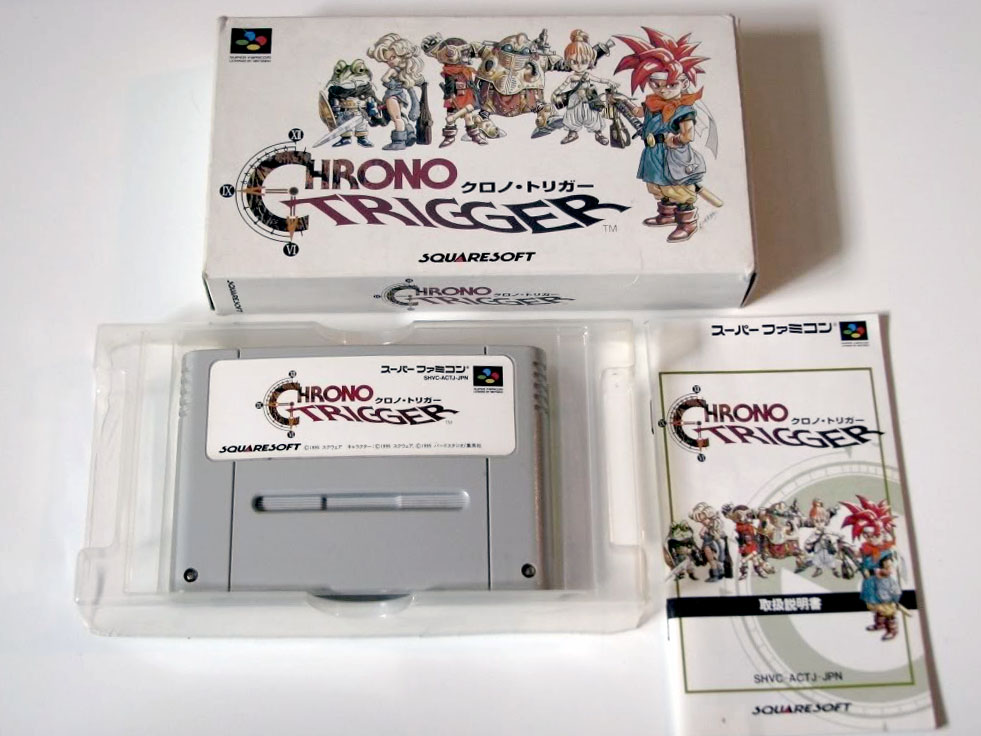
\includegraphics[width=0.5\textwidth]{gamecart}
 \caption{SNES Game Cartridge, 1995}
\end{figure}

\section{Community Based Prototype Design with Dames Making Games and Bento Box-Miso: Overcoming Imposter Syndrome}

In order to refine screenPerfect to a tool for popular use, rather than a specific engine requiring a technician, I partnered with game::play Lab, Dames Making Games and Bento Box-Miso. We collaboratively organized a game jam - a type of design charette, intended to produce demonstratable games in a compressed window of time - that would both test the tool and introduce new game makers to the possibilities of FMV.

The critical theory that underlies this practice is a combination of French poststructuralism - H\'{e}l\`{e}ne Cixous in particular - and contemporary writing on video games and the history of women in technology. By producing the software and content with the input of a local feminist collective, Dames Making Games (\url{http://www.dmg.to}), and as part of a wider feminist research network (SSHRC-funded Feminists in Games (\url{http://www.feministsingames.com})), I have grounded the work in a social justice driven practice which encourages women to take part in their own lives by learning how to interact with machines and communicate with the broader world.

Dames Making Games' mission is to organize women-focused game jams and support women gamemakers. New, straightforward game-making tools provided with the intent to reduce the barriers to producing a game or interactive work, shifting the focus from frustration with game engine's normal assumptions about design to an emphasis on the user's content. By removing barriers such as the requirement for complex scripting, we hope to expand the diversity of experience that can be expressed by new game-makers. 

This is an explicitly feminist goal, derived in part from H\'{e}l\`{e}ne Cixous' "Laugh of the Medusa," in which she describes the necessity of women writing to produce themselves. Cixous' concept describes a space where women required to write, even using imperfect language or tools, least they be written out by the dominant voices that surround them. The \textit{écriture féminine} is also about insists on rebellion with a sense of play, which I find resonant with the practice of feminist, open game jams for learning and self-expression \parencite{cixous}. 

The embodiment emphasized by Cixous is tied to display of personal narrative. Whilst many game works wish to leave the body behind, or optimize it to an ideal form in a play avatar, almost all of the games produced at NoJam 2 had a strong association to the body. Max Lander's \textit{PornGame} explored what it means for a computer to desire interaction, in a sexual sense. Brittney Oberfeld's \textit{OM} explored the embodiment of consciousness and a desire to "slow down," Kate Whyte and Kara Stone's \textit{Cyborg Goddess} presented an adventure through the loss of a leg and the replacement with supplementary systems to become a cyborg or a goddess. \textit{Grimoire}, by Katie Foster and Mikayla Carson, detailed a woman's descent into madness following the discovery of an ancient text.

This seems to be a refraction of the ability of code to make the written tangible.  When you touch a screen, writing – interpreted or compiled – controls what happens next. In this context, the \textit{écriture féminine}can involve a physical change in the environment. The ideas are vividly expressed in relationship mainly to sexuality but desire runs deeper than that: desire can include the desire for agency, for authority over oneself and one's life, or to be seen as competent even by oneself. In this Cixous provides a resistance to imposter syndrome.

Imposter syndrome is common in technological fields, where women form a small percentage of professional game developers - some estimate as low as 4\%, where IGDA numbered 9\% in the last public study released - in 2007 \cite{igda}. Despite this, women consist of a larger percentage of the gameplaying public. The ESA states that women form at least 31\% of the game-buying public, almost double the number of teenaged males \parencite{esa}. The gap between developer and player implies that it is important to provide a way to encourage women to express themselves in this new game form, least women be seen as an alien construct within technological fields. 

\section{Prototype Development: Hardware Installation and Display}

The final section of this paper addresses thoughts on hardware installation and the display of digital works. digital works are difficult to maintain and display because they frequently rely on external systems, such as the public internet, to be consistent and always available. This has proven to be challenging in practice. Rather than relying on a central remote server, in this chapter I address reasons to provide solid hardware in an appliance format for application display, rather than relying on external resources that may or may not be available. 

This chapter is perhaps the most politically informed, as Chapter 2 is informed by the idea that artists should be permitted control over their works and encouraged to produce works using contemporary media. The production of affordable, repeatable installations based on the not-for-profit Raspberry Pi platform means that artists who have participated in web application game jams can then own their own works in the form of common memory and display those works with minimal personal outlay on hardware. This section also asks that we consider our reliance on major internet corporations and how we might separate the computers we use to produce art from the computers we use to serve that art to our audience.

Chapter 4 also presents a number of display scenarios that make use of interesting contexts that do not have ready access to major power or consistent internet. It also presents the idea that the context of the display can extend the value of the work in meaningful ways.

\clearpage
\thispagestyle{fancy}\lhead{Chapter 1. \emph{A Better Time-Based Installation}} 
\begin{figure}[!ht]
 \centering
  \includegraphics[width=\textwidth]{DevelopmentFramework}
  \caption{A method for realizing artist-led technical collaboration.}
\end{figure}
\newpage


% Chapter 2
\setstretch{1}
\chapter{Artist-Led Technical Collaboration}\thispagestyle{empty} % Main chapter title

\label{Chapter2} % For referencing the chapter elsewhere, use \ref{Chapter1} 

\lhead{Chapter 2. \emph{Artist-Led Technical Collaboration}} % This is for the header on each page - perhaps a shortened title
\setstretch{2}

\section{Design Research: Artist Collaboration}
screenPerfect began with an artistic collaboration, where as a programmer, I worked closely with an artist to reproduce the technical elements of a working practice in order to make it available to other artists in a similar field. This specificity allowed us to develop a very simple tool that solves a minimal set of problems in a tidy fashion, while expanding the repeatable part of a single artist's process - the idea of how linked videos \textit{should} connect together on multiple screens - to a tool that can be used by other artists. Arts-led research promotes a point of view distinct from the typical business-forward viewpoint, preferring to ask "how might we" than to say "this is how we will." As a developer, it can be difficult to tie work to a given set of problems, or to ensure it has value to an audience outside oneself. Therefore, collaboration gives access to a set of problems that may seem easy but are frequently technically complex and challenging - and therefore rewarding. 

\section{Software Development Methods: Agile}
The agile method of software development is based on the Agile Manifesto, much as the underlying feminist elements of this project are based on the Cyborg Manifesto and Cixous' manifesto for \textit{\'{e}criture f\'{e}minine}. Agile is a response to previous software design practices, called "Waterfall," where software frameworks are laid out and heavily documented in advance of production. Waterfall methods are popular in major software companies, which rely on extensive documentation to communicate between business units. Waterfall emphasizes planning over software production or delivery deadlines.

The idea of agile was described in 2001 by a group of software developers \parencite{agile}. By using an agile practice of responsive, user-centered design, screenPerfect's interaction model was designed through a series of discussions with key stakeholders, followed by iterative code revisions to a rough first prototype. This can be seen as a hacker-oriented means of development, reflecting Sadie Plant's statement in Zeros and Ones that reverse engineering - "starting at the end, and then engaging in a process that simultaneously dismantles the route back to the start" \parencite{plant}. Agile specifically emphasizes individuals and interactions over processes and tools, working software over comprehensive documentation, customer collaboration over contract negotiation, and responding to change over following a plan \parencite{agile}. 

The screenPerfect development process emerged from a series of linked videos on YouTube, as laid out by Hannah Epstein. We then reviewed strengths and weaknesses of this model: the ability for a large audience with public interlinked video files but the downside of long load times and ads on pages detracting from the video content. In addition, this required uploading films at low quality to a remote server. From the initial prototype, we asked how the process could be improved, particularly for an exhibition context. 

The game processes laid out in Youtube were converted to a "how might we" - a series of static files presented as interactions in still film. Hannah Epstein laid out an idea of how the video screens should work together. I confirmed that this system was theoretically possible using websockets - a communication protocol - loaded into a Node.JS application. From there, I wrote a Node app that served basic video files to multiple browser screens simultaneously. This started as a chat application, serving text to three screens simultaneously over websockets. We then replaced the text with video files, layered a control structure over the videos using plaintext JSON files to replace a reliance on a database structure.

A database was not originally required for \textit{psXXYborg}, the original game built by Hannah Epstein using screenPerfect, or later games using that exlusive engine, because installing a database is an additional step that nontechnical end users cannot be relied upon to find straightforward. Every step of the development process was intended to result in code that is legible to anyone who can read javascript, while being absolutely straightforward to use for a nontechnical video author. 

In development conversations, it became clear that YouTube, in addition to having many distracting advertisements, was very slow to load. This is a problem with reliance on external networks: they cannot be as fast as locally served files. Epstein specifically emphasized speed, smooth loading, and video based in static rather than streaming or live files. These needed to be served within a closed environment to an attentive audience. 

Scripting languages are especially good at this type of development work. I reached out to other developers and asked how they would solve this problem. They came back to me with a variety of answers - some used PHP, some used Python, all of them relied on JS for their front end. In researching different ways to solve the basic problem - passing a variable back and forth through wireless technology to select two on-screen videos at almost the same time - I discovered the Node.JS software framework, a software package designed to permit developers to use Javascript on both the server and client side of a web application. From here, I designed a client-server-control model - Figure 3.1, the screenPerfect Software Communication Model. This relied on an interlinked system of hardware and software designed to respond to what resources it found available in its load space. 

Epstein relied on the h.264 format for her video production, which necessitated an early reliance on the Safari web browser, as HTML5 video does not yet have a settled public codec at the time of writing. Due to conflicts relating to codec patenting, one of many such conflicts that underly the "free" internet, Safari supports H.264 where Chrome supports webm via the V8 engine, the same engine that supports the Node framework. Webm is a compact video format, which results in smaller file sizes and lower bandwidth costs, which eventually affects both load time and playback lag on client machines. 

Figure 2.1 describes the ultimate screenPerfect program code flow, which relies on an always-open two way communication channel based on the relatively novel websockets communication protocol. Essentially, on software boot, a given browser loads a client window and a control window, which open a channel to the server and a passthrough to one another. When something changes, the other channel - always open - displays that change to all paired clients. What is being changed in this case is what game data is dynamically loaded to a single screen at any given time. The flow chart describes how that software's communications patterns travel on a user interaction with a given touchpoint.

\clearpage
\begin{figure}[h!]
 \centering
 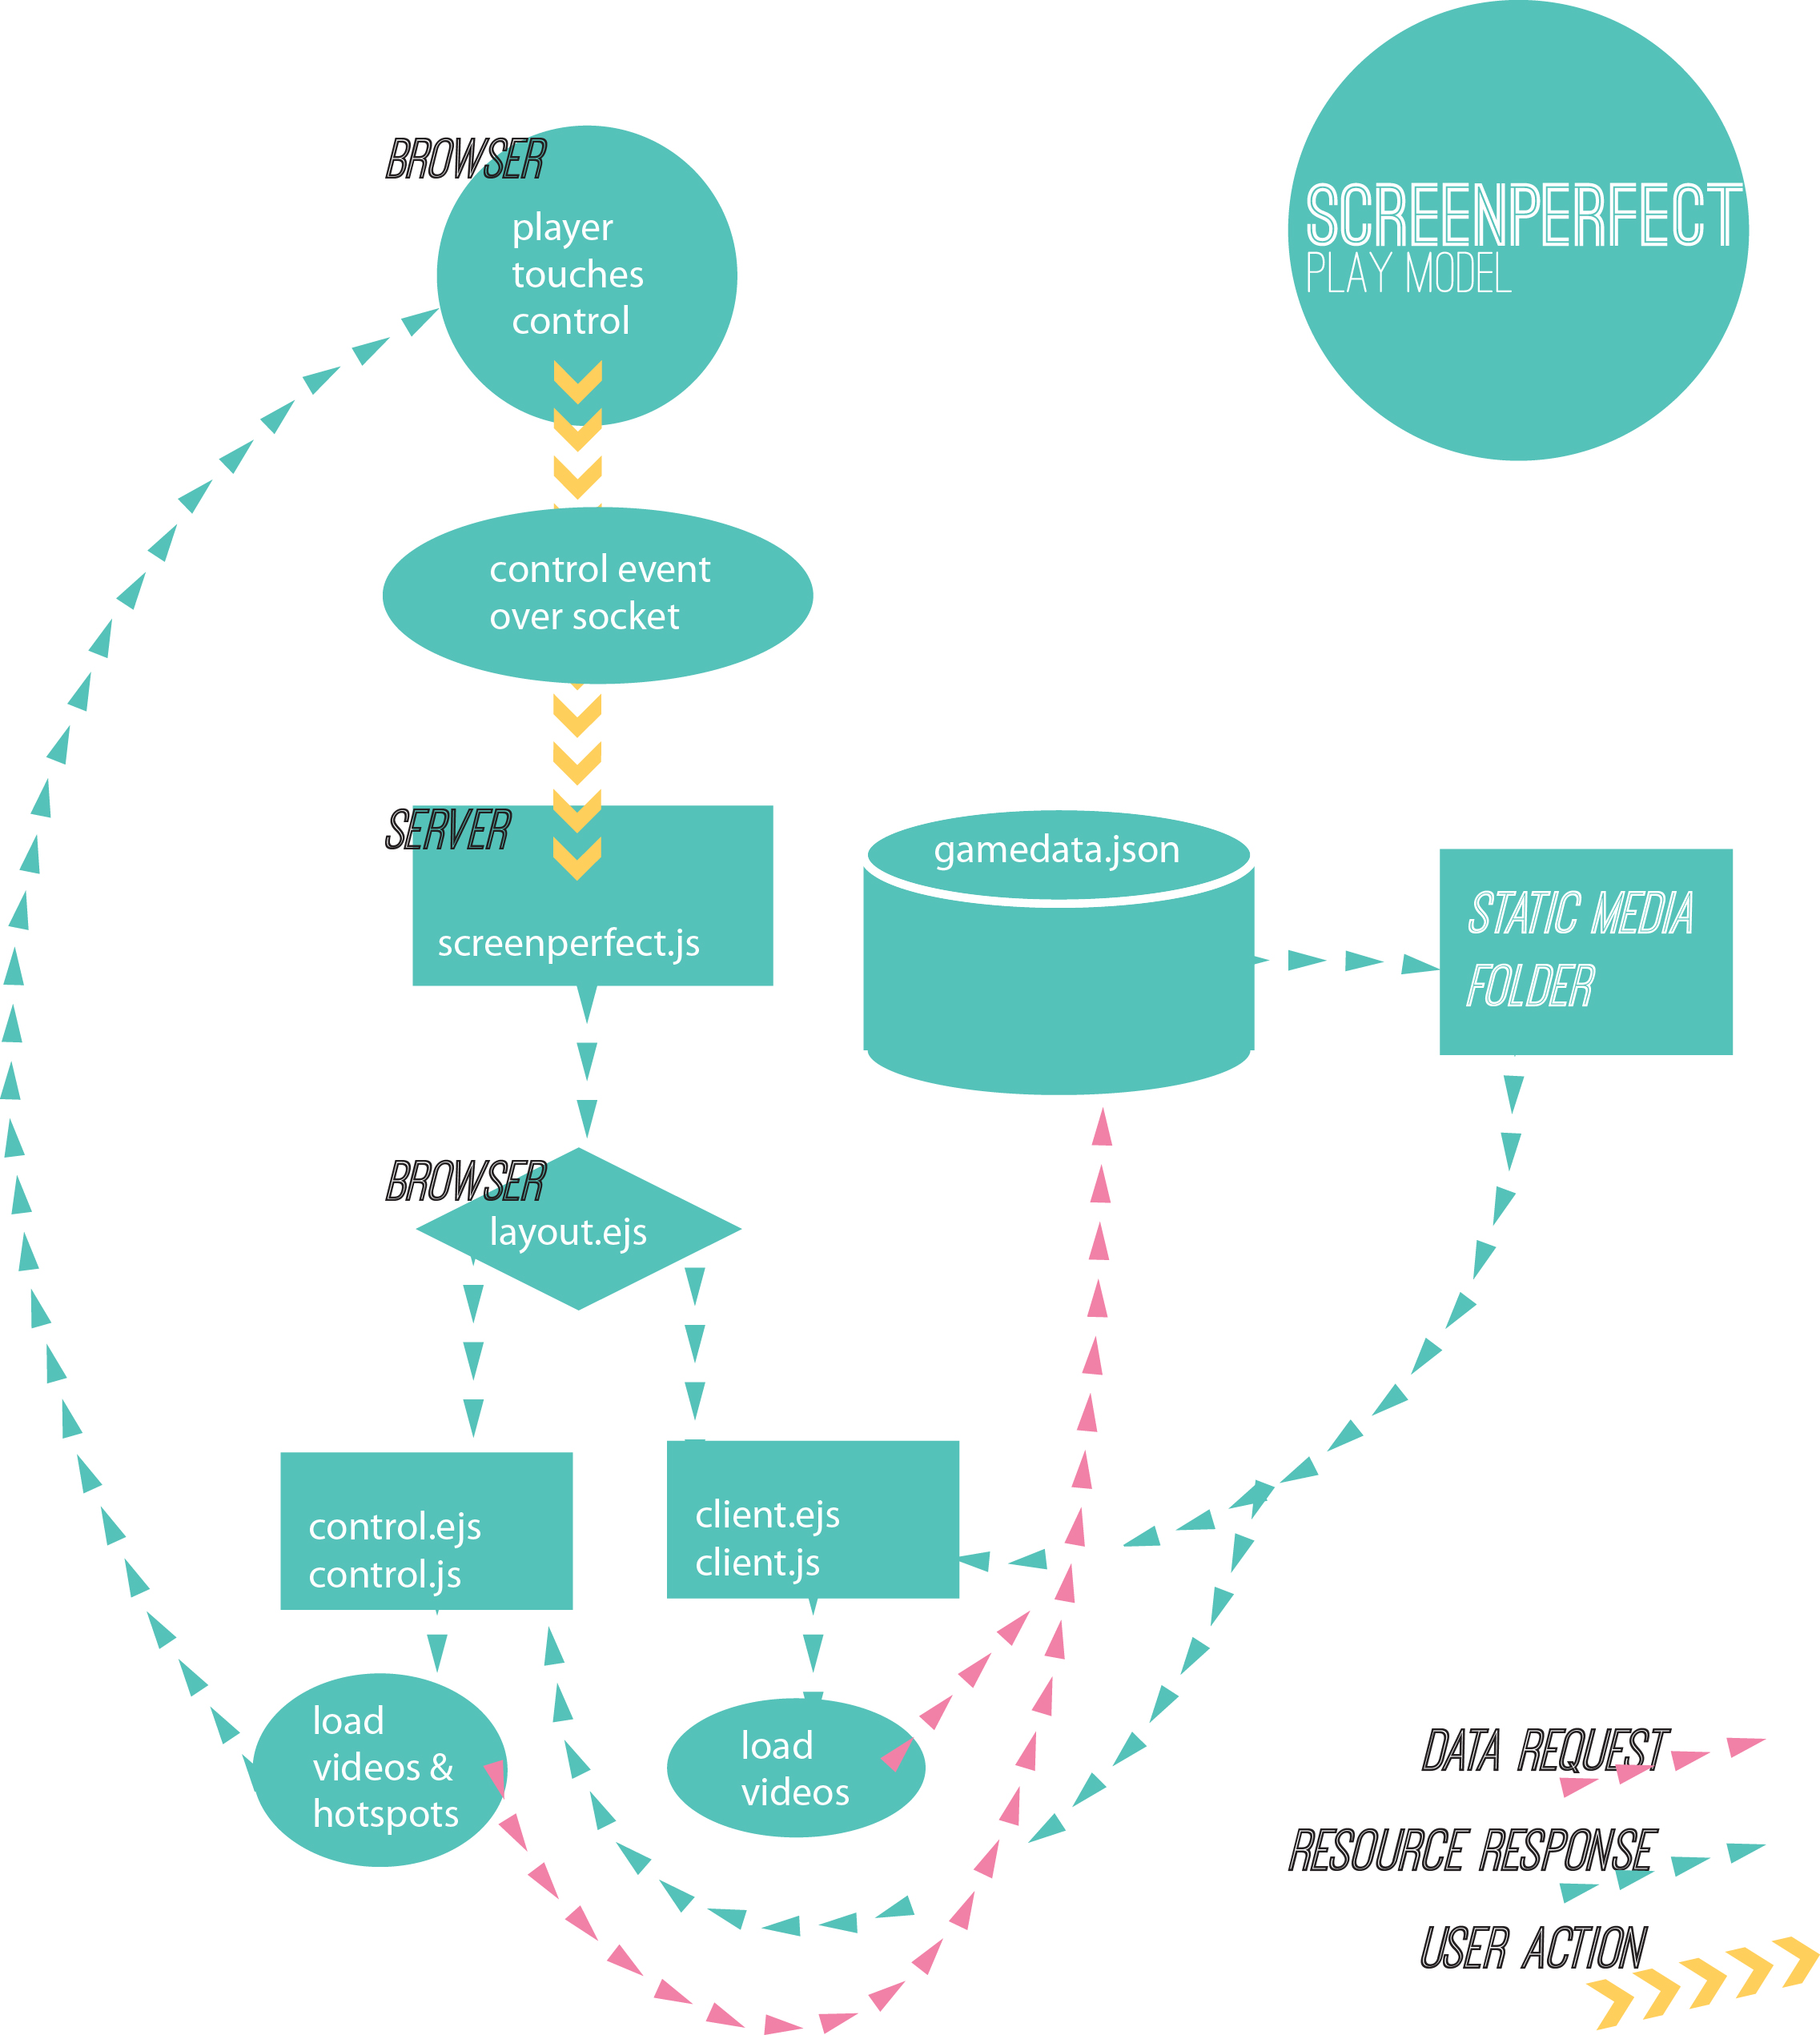
\includegraphics[width=\textwidth]{spCodeFlow}
 \caption{screenPerfect software communication model}
\end{figure}
\clearpage

\subsection{Full Motion Video Games and Mobile Interactive Screens}
FMV (Full Motion Video) games are an old format, relatively speaking. FMV began almost as soon as chapter selection became available on the laser disc systems of the 1980s, with 1983's game \textit{Dragon's Lair} by Rick Dyer and Don Bluth, the first entry in what would become a strange sub-genre. FMV was successful through 1984 but quickly failed due to the expense of laser disc systems and the relative cost of game development and play. The 1985 Halcyon system cost \$2000 - adjusted for inflation, \$4,347.88 in 2014 - and offered only two games. The most well-known FMVs outside of \textit{Dragon's Lair} are \textit\textit, released in 1992, and \textit{Phantasmagoria}, from 1996. \textit{Night Trap} went on to become part of the congressional hearings of offensive video game material along with \textit{Mortal Kombat}, the first widely popular fighting game to allow people to rip out one another's spines. \textit{Phantasmagoria} was better known as the first adult-oriented game released by Roberta Williams, famed for her involvement in Sierra's \textit{King's Quest} point-and-click adventure game series \parencite{encyclopediavideogame}.

FMV and branched narrative games differ from cartridge-based action games in that they do not typically feature the same immediate feedback of a score going up and the instant player controls of a more typical 2D or 3D action game. Instead, players select what will happen next at key intervals. Older games are easy to display, so long as working hardware can be found, because they rely on consistent materiel for installation. Digital interactive forms, particularly those on the internet, live in a more malleable format. They can change, or be taken down, at any time. The gameplay experience of a console game can be had even when disconnected from the internet – in fact, the Nintendo 3DS, a pocket console, outsold every other system on the market in 2013. It is speculated that its success is due largely to the fact that the 3DS is a portable system that does not connect to the broader internet unsupervised \parencite{3dssales}. This reliability is something that is rare to find in more complex computers: sometimes, as argued by Don Norman in "The Design of Everyday Things" \parencite{norman}, it is best to have a single thing do one thing really well. 

FMV games remain interesting enough to engage fans. This is partly due to the well-documented nostalgic appeal of certain forms of entertainment, digital games in particular sparking sites such as videogamenostalgia.com and hashtags on Tumblr like \#videogamenostalgia or \url{http://fuckyeahchrono.tumblr.com/}. FMV have been recreated using Youtube and preserved from laser discs and DVDs \parencite{laserdiscarcade}. Phantasmagoria can easily be found in complete playthrough on Youtube, where the annotation system makes recreating a point-and-click environment trivial (\url{https://www.youtube.com/watch?v=oAXC-MwfpHA}). Nonetheless, they were heavily systems-dependent and are tricky to develop, given the difficulties surrounding copyrighted video works and public distribution - how to transmit something that contains so many different pieces of video information?

Another example of portable electronic interaction is the smartphone. Initially this technology seems not so great for bringing people together in the same space, as the privacy of the phone has been seen as undermining or distracting. It is possible to see this instead as a source of potential: people examine things one-on-one with their devices and then will share them with their peers.

Smartphones are inherently private systems - a category of hardware referred to as a "personal device" - used in public places. Personal devices have all kinds of content on them, from games to e-mail to tax returns. Apps, paid for and downloaded, are understood to be private even when their terms of licence imply that they are the sole property of the developer. Websites are public places one can "visit" on a phone, an external resource supplied to a personal locale. This leads to a set of assumptions on behalf of interaction developers: an application is a private thing, paid for, and downloaded to a private space within the phone, whereas a web page is a public resource that can be viewed in private on a phone. A smartphone is also a single encapsulated controller, with all necessary inputs provided by its touch surface. For interactive artwork, this means that some assumptions can be made.

The first is that the audience of an interactive art piece is likely to be familiar with how to interact with a touchscreen but also may be distracted. It cannot be assumed that they will download or pay for an application sight unseen for the sake of art, because that would constitute an expenditure of resources without reference but they can be asked to go to a web page. People commonly use their phones in public. Therefore it seems reasonable to ask them for the minimal engagement of looking at something specific, this time art served only within the gallery. 

There are already games that aim to subvert this separation. Systems have been built to take advantage of the power of pocket computers. A notable effort is "Spaceteam," \parencite{spaceteam} a ‘Simon-Says' game for teams of up to four players. The application pairs to itself across phones by using a common network connection, having players in the same physical space cooperate to pilot a star ship. This allows players to make use of a device with which they are already comfortable to cooperate and share an experience.

This shared experience makes it possible to privately host a public space. A private host is a computer that is unreliably connected to the broader internet - perhaps occasionally, perhaps not at all - which serves an application using technologies that make it appear to be part of that internet to people who access the resource using their phone. These are web applications, served in private, to a public but small gallery space, to preserve the context of the application while relying on the user's own resources in the form of a phone to give the work a personal context within the public-private site. In this way, a private site which cannot connect to the broader internet can take advantage of the design model of internet communication to serve works without them being decontextualised to anyone who wishes to navigate to them more broadly.

In this way, web art is no longer the broad exploration of net.art but becomes instead a preservable, repeatable installation.

screenPerfect, a web application served locally, takes advantage of an assumed set of smartphone users in galleries having access to the internet in their pockets. The internet is both bigger and smaller than the wider network – the internet that includes Google and other multi-national internet corporations. Rather than relying on the external resources of remote servers, screenPerfect provides a private wifi point and what is called a "captive portal" to let players pair with one another and the server, control a large screen, and interact with a piece of video art in a localized area. This means that an artist can control the exhibition space for their work, design the experience of the work, and ensure that their audience will experience the work in a specific context. It also ensures that technicians can access the underlying engine should something go wrong during the installation.

\section{Game Engines}
A game engine is a collection of software designed to make it possible for a team of artists, developers, musicians, and producers to work together to produce a complete digital experience. Traditionally, game engines are used to produce 2D or 3D experiences using assets such as 2D sprites or 3D player character/interaction models, backgrounds, interaction assets - crates, for example - music, and scripts in a programming language to tie all of these together into gameplay. 

Some popular professional engines at the time of writing are Unity3D, which features native mobile integration and ease of scripting in both Javascript and C\#; Crytek, which comes with many high-end 3D resources preloaded for high definition graphic support; the Unreal Engine, which is quite stable and useful to experienced teams that prefer more control over their work.

There are popular hobby engines that de-emphasize programming as well, such as GameMaker, which is prized for PC compatibility, Game Salad for OSX, and Construct 2, which is PC-only but has a powerful engine to manage game physics and interactions. These engines all assume a certain type of player interaction: they are designed to enable designers to produce specific types of games, such as a "shooter" or a "platformer," similar in style to the \textit{Call of Duty} franchise or Nintendo's \textit{Mario} series. The interactions available are easily understood as a language of action by their players, provided players have previous experience with digital gameplay.

\subsection{Twine}
Twine is a game engine that allows designers to build HTML5 text narratives that branch into a choose-your-own-adventure game. screenPerfect was inspired in no small part by the popularity of both Twine and video on the internet. Twine encourages expressive type styling and elements of multimedia, including music, and game screens but does not require these elements for a complete interactive narrative. Twine did not yet support video narratives in 2013.

The Twine engine was popularized by DIY gaming celebrity Anna Anthropy in her 2012 book \textit{Rise of the Videogame Zinesters} \parencite{anthropy}. Anthropy's book calls for a dramatic DIY practice to articulate personal experience in video games. She strongly promotes Twine as an easy way to begin the effort of designing personal games. Since then, hundreds of Twines - the adopted term for narratives built in Twine - have seen release.

\subsection{Multiscreen Video Technology}
Dual screen technology, or more accurately, multi-screen synchronous web technology, is one of the big new ideas being heavily backed by Google in 2013. As a consequence, its Chrome browser has been designed to support software developed with a specific suite of frameworks, many of which are wholly supported by Google. 
This being said, Google supports Node and Chrome both, so multi-screen technology using web browsers is open to people for no more investment than a new programming language. screenPerfect relies on Node.JS, which is based on Google's V8 engine.

The architecture of screenPerfect is wholly new but the concept is based on the Dataton Watchout system, which encourages producers to develop large multi-screen single video experiences on custom hardware. Dataton Watchout costs approximately \$40,000 dollars per installation, which makes an inexpensive alternative appealing from a creative standpoint. screenPerfect permits people to use existing hardware to synch multiple videos to one set of controls. This is also distinct from another related tool, ChromeCast, that allows people to wirelessly pair a television with a touchscreen for control and consumption of the touchscreen at a larger size. ChromeCast requires an ecosystem of development that is presented as inclusive chiefly to those already invested in the startup scene. Therefore, these tools have been built from a position of inclusivity. By releasing them through a group of largely non-technical artists, I have chosen to pursue a research path that deprivileges the role of the technology compared to the role of the artist within a given system.

\subsection{Licensing}
One of the ways these problems are dealt with is through licensing. The Creative Commons at creativecommons.org expresses their mission as follows: "Creative Commons develops, supports, and stewards legal and technical infrastructure that maximizes digital creativity, sharing, and innovation." It is therefore an appropriate open standard licence for creative practice. A preferred licence for software development is the MIT Licence, which is closer to the Gnu Public Licence but does not preclude making money from one's open source work. 

\subsection{Science Fiction Inputs}
My own idea for how this project would work is derived from Cory Doctorow's \textit{Pirate Cinema}, which features a scene wherein characters climb trees then use projectors already built into their phones, assemble a movie theatre from nothing more than sheets and ropes in the trees \parencite{doctorow}. I feel this sort of mesh-networked sharing is much more likely than a continued reliance on the surveilled internet for sharing copyrighted and copyrighted- material derived works. Since I could not find a system that would permit this type of sharing on the internet, I felt that this project would provide a good opportunity to build one.

\section{Code as Context-Sensitive Writing}
As a creative project, code is a tricky thing to pin down. It must say something structurally, yet it reveals the internal architecture of its authors. Programming leaves loose ends. An excellent piece of software is likely to require input from a wide array of specialists in graphic design, interface development, and logic. There is an inevitable tendency to produce flaws - bugs - that cause the program to fail. Once complete, it is likely that finished software will fall out of fashion. Just as there is no way to call a piece of writing finished, because another word can always be added or cut loose, code is subject to scope creep. 

Code lives, like writing, in context and within an ecosystem. Code answers to its context. As Alexander Galloway says in his book "Gaming: Essays On Algorithmic Culture," without the machines that run it, code is without consequence \cite{galloway}. Within those machines, code may have a concrete effect on the world around it. For that reason it continues to be valued. To code is to attempt to write a way of addressing the world, a single way that must take into consideration all the assumptions of people who tried to address the world before, and, with future-proofing, the world after. 

\section{Software Design}
A software interface is the part of the software that a person interacts with directly where a software engine is the part of the code that detects and defines what a computer can do with that interaction. 
The interface of software is just as important as the engine, however, because a poorly designed interface will confuse a user thereby rendering the experience of using the engine potentially opaque. 
screenPerfect's roots are as a software engine, which takes user action and then does things with it. The user interacts with the interface that speaks to the engine which then returns values to whichever interface the user has selected.

\subsection{screenPerfect Engine|Interface Layout}
In the case of screenPerfect, the interface is laid out in three parts. The first part is the setup screen, the second is the control screen, and the third is the generic client screen. The setup area is by far the most complex area. It is used by game designers to load their media to the database and lay out the links between those files. This is the essence of a game made in screenPerfect: which choice will a player make to navigate the system as designed by the artist?

The further screens are the client and control screens. screenPerfect supports up to ten client screens and ten control screens, although the interface only exposes a polyphony of client windows, while restricting artists to a single control set for simplicity's sake.

The layout of screenPerfect's editing tools did not work very well for authors who were not already part of the prototyping process. Therefore, as part of the extension of the software for NoJam, Bento Box-Miso reauthored the editing interface of the software. 
The final editing layout is clean, though less expressive than the original design. Rather than hidden tabs, everything is displayed on launch. This permits authors to see their video files during the entire game editing process, which greatly speeds game creation. 
What follows are screencaptures of the pre-fork game jam variant of screenPerfect.

\newpage
\begin{figure}[h]
 \caption{screenPerfect NoJam editor, Asset Population tab.}
 \centering
 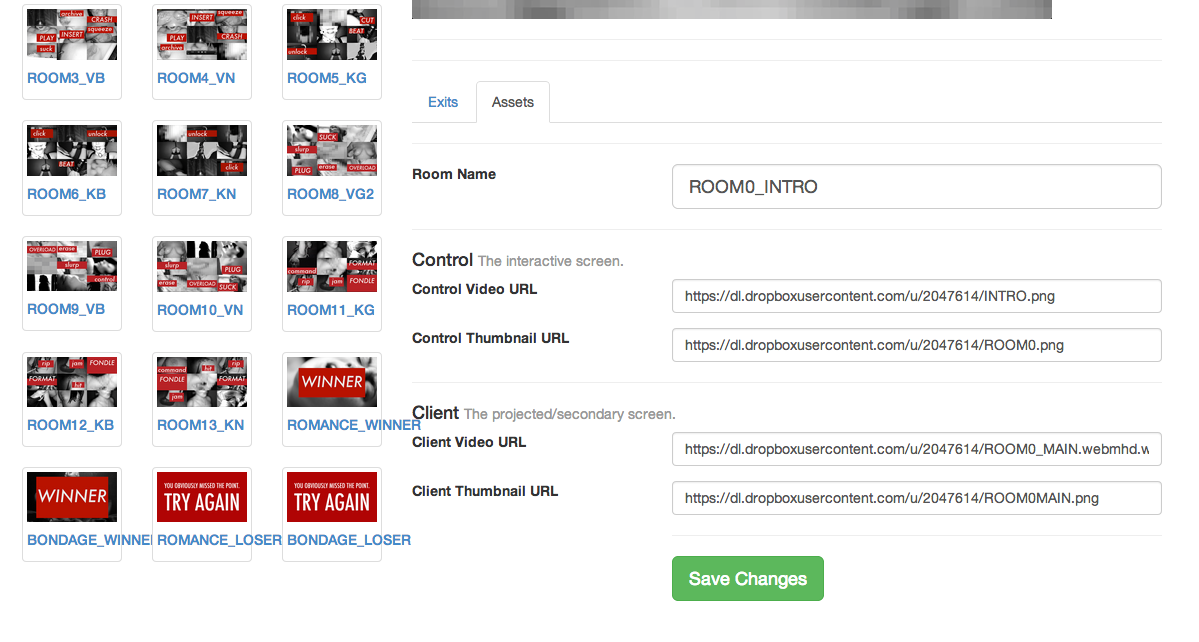
\includegraphics[width=\textwidth]{editSoftAssetTab}
\end{figure}

\begin{figure}[h]
 \caption{screenPerfect NoJam editor, Exit Population tab.}
 \centering
 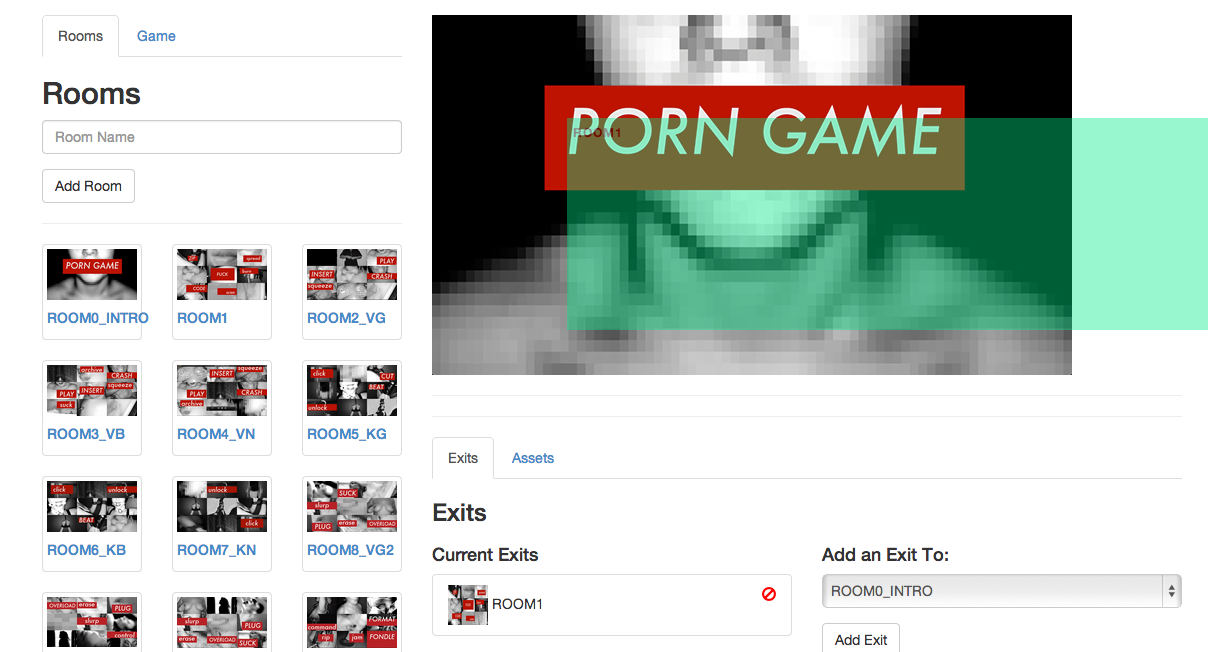
\includegraphics[width=\textwidth]{editSoftExitTab}
\end{figure}

\newpage  
% Chapter Template
\setstretch{1}
\chapter{Industry Engagement and Community Based Research}\thispagestyle{empty} % Main chapter title
% and Design Research: Community Collaboration in Software Development
\label{Chapter3} % Change X to a consecutive number; for referencing this chapter elsewhere, use \ref{ChapterX}

\lhead{Chapter 3. \emph{Industry Engagement and Community Based Research}} % Change X to a consecutive number; this is for the header on each page - perhaps a shortened title

\setstretch{2}
%-----------------------------------
%	Software Design for Game Jam
%-----------------------------------
\section{Theory and Politics}
Cixous' "Laugh of the Medusa" predates the computer age but perfectly and predictably describes the opportunity present in programming - which is a form of writing - within "Laugh of the Medusa":
\begin{quote}
"Write, let no one hold you back, let nothing stop you: not man; not the imbecilic capitalist machinery, in which publishing houses are the crafty, obsequious relayers of imperatives handed down by an economy that works against us and off our backs; and not yourself." 
\textit{\parencite{cixous}}
\end{quote}

In this passage, Cixous chides her readers for not giving themselves the permission to write, because writing is reserved for those who might be published. This is similar to game-makers who might not produce, merely because the engines are closed, or distribution unlikely. Women have a long history in technology.
Ada Lovelace, daughter of Lord Byron, has been identified as the first programmer \parencite{plant}. The ability to put rules in order, to work backwards and forwards from a desired result all along the path of the machines, is a characteristic much sought for in both programmers and game designers. Both roles are responsible for rule systems that will dictate a predictable result.

In a straightforward way, ladies may not possess uncomplicated positions of economic advantage within a patriarchy: to do so would be to "have it all," a famously complex desire which is reanalyzed every year in popular press, most recently by Anne-Marie Slaughter in \textit{The Atlantic} \parencite{slaughter}. The balancing factor is housework and the social expectation of family, which still places a gendered burden on women to produce both children and home. This system of expectations, divided between household and the potential for earned income, re-creates itself in each new trade as it arrives, in fields as far apart as World War II factories \parencite{summerfield}, Victorian mills \parencite{baskerville}, and lately, code factories in Manhattan and San Francisco \parencite{newdomestic}. Computers have quickly become a good job with a good chance to better one's life, and just as quickly have moved from being women's work to being a heavily masculinized field \parencite{ensmenger}. This is unfortunate, as it is presently popular to assert that in the future, there will be two types of lives:

\begin{quote}
"...those who tell computers what to do, and those who're told by computers what to do."
\textit{Marc Andreesen, Andreesen Horrowitz 2012.}
\end{quote}

Within such a system, people discouraged from understanding technical roles, their uses and disuses, could then be expected to be mainly among those being told what to do. This does not seem to be a pleasant future, inclusive and positive for all people, and as such, perhaps the vision could be broadened.

Computers are a tool, and the way that the tool is presented, held, and used, dictates the results. A computer - a machine for automating an interaction - can be made simpler or more complex to use. The device may be changed to an amplifier of force, made more opaque, or made clearer for those who choose not to learn to code but can still understand systems of logic. "If this then that" is not a complex instruction set. The complex instruction sets should, rather than being encouraged to control people, be developed to be under the control of people.

screenPerfect has been designed to present the idea that a simpler system will result in a more diverse body of work. It dictates nothing whatsoever about content, presenting instead a simple system of switches that permits the author the broadest possible control over simplified interaction sets. It is implied that these interactions will lead to a coherent narrative but it does not dictate what content an artist might use. The voice of the artist is brought to the forefront of the work, rather than the voice of technology.

By simplifying the process of game design and displacing its nexus from the computer to other design tools, technology is repurposed to be one tool among many. This displaces technology's primary position and refocuses the work on the intent of the artist. This is an implicit system of resistance to the narrative of technology: people can once again tell computers what to do, and extend themselves via their tools.

\section{Cixous, Embodiment, and the Game Jam}

Many of the participants of the game jam produced, with the simple yet powerful tools provided, narratives centered on their own embodied or disembodied experience. The only group to resist doing this were the younger OCADu students who came to the jam via a game design practice, rather than a filmmaking, animation, photographic or other digital interest.

Of the games produced and finished, \textit{PornGame} by Max Lander is directly about the experience of sexuality as it applies to a machine. Grimoire is about a loss of personal agency following the finding of a "grimoire" or textbook. \textit{Kill Fuck Marry} was about bad decisions when it came to dating and sex, \textit{OM} about a practice of embodied mindfulness, and \textit{Cyborg Goddess} went straight to Donna Haraway's "Cyborg Manifesto" in a literal interpretation. \textit{Glitch.95}, though mainly interested in the glitch aesthetic, is a depiction of the beginnings of an internet relationship. \textit{Puppet Story} is about a genderless creature coming to life, Pinocchio-esque - or perhaps more Galatea, though that is projection.

This is simply an observation but a comparatively high number of personal and body-centric stories came from this jam, which was nominally about the use of a tool to express a new format of interaction software. This seems tied to Cixous' assertion that "You can't talk about \textit{a} female sexuality" and her immediate follow-up that "time and again I ... could burst forth with forms much more beautiful than those which are put up in frames and sold for a stinking fortune" \parencite{cixous}. This is the core of what games critics are discussing when independent games, or new art forms of any type, are being spoken about publicly - the potential expression outside commercial benefit. Cixous's conception of masturbation and writing as a unified activity practiced in secret can be easily associated to the idea of imposter syndrome, the thought that one could not possibly be "good enough" to break into a creative or high-level industry \parencite{imposter}. 

Imposter syndrome is a major problem in the technology industry, and in games even moreso: because code is a high-level creative practice, with a great deal of material reward when done properly, and games are similar, the stakes are high. I have conflated games and code because both are systems of organized rules: game design is a type of code, where one purses conditioned response and engagement through good user experience design. It is easy to back off from both practices or to pursue them exclusively as a hobby, rather than believe in them as a trade. Does one wish to join the commercial order? Is it necessary to be validated, to have commercial success, or is it simply another demand on the work, that the work sell to prove that it is fundamentally worthwhile? These questions are outside the scope of this paper, although my personal opinion is in line with Cixous: whether the money follows or not, a plurality of voices in any creative practice is important for its own sake.

Cixous' throwaway line, of "arid millenial ground to break" seems especially poignant in light of the generational nickname of the jam participants. 


\section{Industry Engagement}
\subsection{Game Jams, A Design Method}
A game jam is a variant on the hackathon, which is a type of prolonged effort at taking an idea from concept to finished product in a limited period of time. Game jams and hackathons are both derived from the design charette or parallel prototyping process \parencite{martin}, a method in which participants rapidly prototype a design idea over a short, intense period of time. Charettes stem from the architecture field, and benefit from the idea of a concentrated sprint of effort to complete a given project in a narrow window, thus preventing the project from creeping too far out of scope. A jam - or hackathon - gives registered participants a common area and space to set up their own equipment and supplies, and a theme. The group members come to the event with an idea and possibly some resources - video files, sound capability and so on - and use the jam time to assemble a game.

Generally, a game jam will produce a panoply of small game ideas with fleshed-out mechanics but simple art and sound design in order to demonstrate a possible path forward for a device or piece of software, which will then be polished at a later date, and presented to the indie community either online or at a social event. Sometimes these works will then go on to be finished commercial products, or are intended for further consumption at major conferences such as Indiecade or the Game Developer's Conference, GDC. These conferences can further the careers of the developers by providing access to funding bodies and publishing houses (whether traditional or online), or in Ontario, the Ontario Media Development Corporation. Other funding sources can include research groups, via research funding bodies. By framing game jam development as research, participants can be released from the need to make commercially appealing works. In the case of Dames Making Games and screenPerfect, funding came from the Feminists in Games project, headed by Jen Jenson of York University, and GRAND FRAGG, a research project dedicated to expanding the diversity of voices represented in gaming. This research funding supported the research goals of this collaboration led by Professor Emma Westecott at the game::play Lab.

Game jams can be time consuming to prepare, as they involve a great deal of communication on the part of the organizers. In order to run a jam, one must open the application period well enough in advance to ensure a large cohort of skilled participants who are likely to be interested in producing content with the available tools, or interested in exploring new tools on offer. Typically, jam attendees have a theme suggested - for example, "Mother May I" or "Snacktember" jams organized by Dames Making Games - and then participants bring their own preferred technology to produce a fast prototype over a weekend.

\subsection{Dames Making Games and Game Jams}
\begin{quote}
Dames Making Games (DMG Toronto) is a non-profit community organization based in Toronto dedicated to supporting dames interested in making, playing, and changing games. In short, we want to build an \textbf{inclusive} and \textbf{engaged} local community of game-makers. Our community isn't women only but it is women-driven.
\textit{from the DMG.to website, accessed November 27, 2013}
\end{quote}

Dames Making Games (DMG) is a community group in Toronto that work to promote women in video games. They have been funded in part by FiG (\url{http://www.feministsingames.com}) and in part by member donations. I am a founding director and advising director with the organization, which has given me ready access to a test audience for my ideas with regards to development tools. DMG uses the game jam method to introduce women and allies to simple game development tools. This provides a straightforward introduction to concepts of computer logic and programming for some people, to video game art development for others, and video game sound production for still others. Some develop system mechanics, some design whole levels or game narratives. 

The point of DMG is to promote access to this field to people other than the 18-to-35 year old males who form the primary demographic for the video game industry \parencite{esa, igda}, in the hopes that a diverse population of game makers will produce a diverse population of games. DMG is interested in screenPerfect as it provides an underlying template for a game-making system that might be easier for newcomers to use than other freely available game engines.

\subsection{Bento Box-Miso}
Game jams require both space and people who are interested in working on games. A themed game jam, such as No Jam 2, which was designed to test specific software, requires a specific audience and support. In order to access that space and community, I worked with the Bento Box-Miso co-working facility in Toronto, with OCADu's game:play lab and Emma Westecott, and with Bento Box-Miso, a development company that runs Bento Box-Miso as a not for profit co-working facility.

Bento Box-Miso is a not-for-profit community coworking facility that serves as home for both Bento Box-Miso, a local development hub, and the Dames Making Games. It is also the hub of a great deal of Toronto's independent game development community. Bento Box-Miso offers professional support and development advice to game developers. I felt there was a good match between their professional skillset and my research interests. DMG regularly run a jam in November and felt that screenPerfect - new software designed to be usable in a short time frame to people with extant skills - would be a good match for the audience associated with the organization. 

Bento Box-Miso was also at the time seeking an engine that could display the capabilities of their new programming language, Daimio, which offers users the ability to reprogram work on the fly in the browser without being a trusted network source. Therefore, I accepted their help and their offer of hosting the jam in return for giving them permission to fork - copy, reproduce, and extend - my engine under their name. 

As a pair, Dann Toliver - architect of Daimio - and I worked together to clean screenPerfect to speak to the Daimio dataflow language. Bento Box-Miso then released a refactored version of the code in time for No Jam 2, so that our participants could get a clean version of the software to work with. This was challenging for me, as it involved a great deal of trust and moved the software away from how I had initially envisioned the user interface (UI). In particular, we needed to scrap an early idea for a branched narrative "tree" display similar to that of the Twine engine, which was not included, although it had been planned all along (Figure 3.1).

\newpage
\begin{figure}[h!]
 \centering
 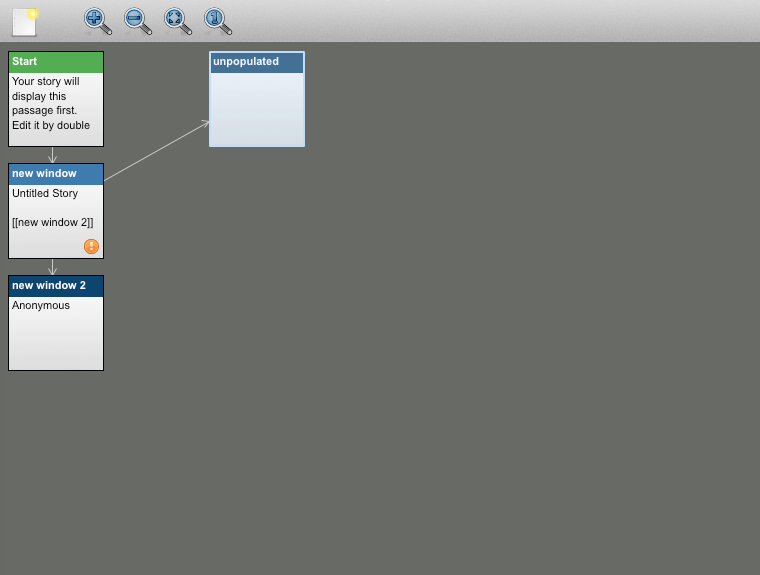
\includegraphics[width=\textwidth]{twineNodeTree}
 \caption{A branched tree of rooms from Twine.}
\end{figure}
\newpage

\subsection{No Jam 2: Video Video}
DMG have a great deal of experience running jams. In addition to a skilled community, the ongoing success of research in the community is dependent on participation by community members' voluntary engagement in participatory research. The premise of DMG is that people learn well by doing something new in a supportive environment and that they can carry the experience of a supportive learning environment forward to effect real change in the game development landscape. game::play Lab is researching the outcomes and process of this type of development practice. By partnering with DMG, I gained ready access to their community and they gained access to my software. One of the most common difficulties with game jams is that the short timeframe can cause a lot of frustration to new non-programmers: they spend a lot of time wrestling with tools, rather than generating the content of their games. This is a theme that came up again and again in research interviews, most notably and clearly presented in Appendix A's DVD support by Team Grimoire - Katie Foster and Mikayla Carson:

\begin{quote}
"I've come to jams three times now and I never do it very well... the new tool caused me to change my concept and execution but not by much. It's learning on the first day if I can make my idea work with that tool and then teaching myself that tool, because usually I have no idea how to use it.... I like the constraints that have been put on the project, since it's made me pursue new things I'd never pursue. ... It's like five rooms, they all hook straight to the next one, I'm not intimidated about putting it into the tool. ... that's what's so awesome, I'm so used to having to learn ALL new skills, every time I jam, and then I get really frustrated and I don't want to do it any more, so this time I'm like 'I know how to do all this stuff already.'"
\end{quote}

The reduction in technical barriers to entry resulted in five complete games coming out of the No Jam process, one of which was exhibited at the Art Gallery of Ontario.

After we received No Jam applications, we went through them to choose participants who seemed interested the theme and the software restrictions, sent out acceptances, ordered food, and set the dates. Applicants were provided diaries to record their working process over the course of the week. The first weekend of the jam consisted of workshops from a variety of specialists to provide direction in how to think about the software and the jam process as research.

The applicants were then sent home for a week to work on their video projects. They were asked to document their ongoing process with one another on a private Google Group. Most participants ignored this request, which left us with relatively little online material.

On the actual weekend, we asked that participants arrive with the majority of their video content and design prepared. There were uneven responses to this request, which strongly affected the ability of participants to produce a finished game by the end of the weekend. I interviewed each group early in the process and then later polled them with informal questions regarding their experience with the software. The interviews are documented in my electronic support materials in named files. During interviews, I asked participants about their background, what they expected from a game jam, their previous experience in game or media design. I also asked whether they found the restrictions of working with the screenPerfect software package useful, damaging, easy, or difficult. The main responses of interest were not about the software at all, although Mikayla Carson clearly stated that as a filmmaker she found screenPerfect much less frustrating than traditional game engines. The responses of most interest involved how people think about producing media, their frustrations with traditional computer work, and their experience with collaborative game practice.

I asked each group to name themselves, talk about their background, and tell me what they expected out of a game jam. Then, if appropriate, I asked what their experience with the software was and how it compared to other game-making engines and software. The interviews with each group proved diverse. Responses are recorded on my electronic supporting materials in the appendices, under the folder "Game Jam Interviews."

The group experience with the software proved interesting. Accomplished filmmakers had a better time with it but the most surprising response was from young, self-identified gamemakers, who rather than exploring what was possible within the context of the software tools, decided instead to try to use them to reproduce existing game types, many of which were totally incompatible with the software design. Of particular interest was the group who tried to reproduce a classic Japanese roleplaying game within the context of video: this did not work so well. The group continued to work on their design even after it became apparent it was unlikely to go well. The game itself remains unfinished but deserves mention as the most unique and possibly stubborn effort.

Despite this, No Jam was a success, with nine groups producing diverse works on ideas such as how to express a practice of mindfulness, how to work with pornography in a way that forces the viewer to interact with what's happening on screen, exploring systematic violence against women, exploring narratives of imprisonment, magic, and in one unique case, permitting a puppet to escape a toy box. 

In setting up No Jam, we did present at least one workshop on the importance of personal narrative in producing creative work, which may have influenced the results. Game jammers mostly described their interest in producing work that was finished. No Jam resulted in at least five "finished" works, which have since been included in several exhibitions around the city, including the December and January Toronto Long Winter series. The finished works can be found on the supporting materials DVD under the folder "screenPerfect games."

% Chapter Template
\setstretch{1}
\chapter{Prototype Development for Display Hardware}\thispagestyle{empty} % Main chapter title

\label{Chapter4} 

\lhead{Chapter 4. \emph{Prototype Development for Display Hardware}}
\setstretch{2}
\begin{figure}[!ht]
 \centering
  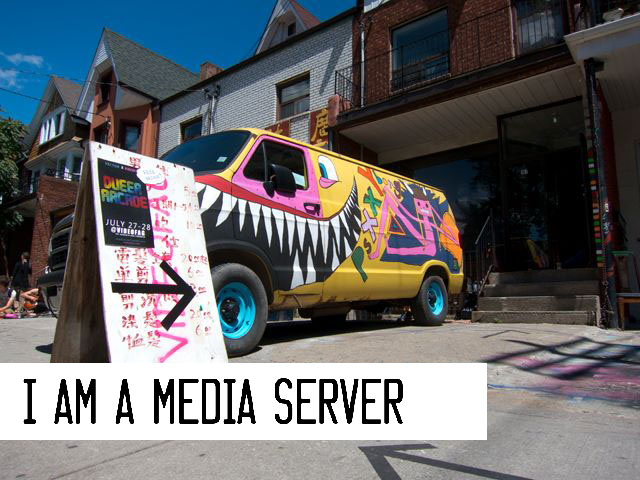
\includegraphics[width=\textwidth]{psXXYborgVan3}
  \caption{Hannah Epstein\\ psXXYborg at VideoFag, 1995}
\end{figure}

\clearpage
\begin{figure}[!ht]
 \centering
  \includegraphics[width=\textwidth]{ServerClientModel}
  \caption{screenPerfect interaction model between client, server, and studio.}
\end{figure}
\clearpage
\section{Client Server Model}

The chart in Figure 4.2 describes how screenPerfect's hardware serves a connection to a local cell phone, while occasionally obtaining software updates from the internet or from a direct upload when the resources are available for that upload. This is a useful model for public exhibition, because it does not require the device to be always-online with access to remote system resources. Instead, the software to run the artwork is stored locally and serves as both its own webserver and its own wifi hotspot, so that users can pair with the device on their own cell phone and interact with the art in public.

\section{Public Installations}
During the course of this project, games made with screenPerfect had many public outings. We installed \textit{psXXYborg} in a variety of spaces. There were a number of design approaches to the construction of those spaces. Hannah Epstein created many variations on space design, in including a straight projection on mylar, a whole-room space that would encompass the user in different projected, linked screens, and ultimately a portable "confessional" booth. The first variant of this is displayed in Figure 4.1, a custom-painted cargo van which we displayed at Videofag in Kensington Market as part of the Queer Arcade with Vector Art|Game Festival as part of their 2013 show (\url{http://www.vectorfestival.org/}).

More recent exhibitions of \textit{psXXYborg} have been built into a tent, which can be more easily displayed indoors. The \textit{psXXYborg} tent has been exhibited at Long Winter in December 2013 and at the Feminist Art Collective's annual conference at OCADu in 2014 (Figure 4.3). This helped to test and refine the list of design constraints for a successful work.

\clearpage
\begin{figure}[!ht]
 \centering
  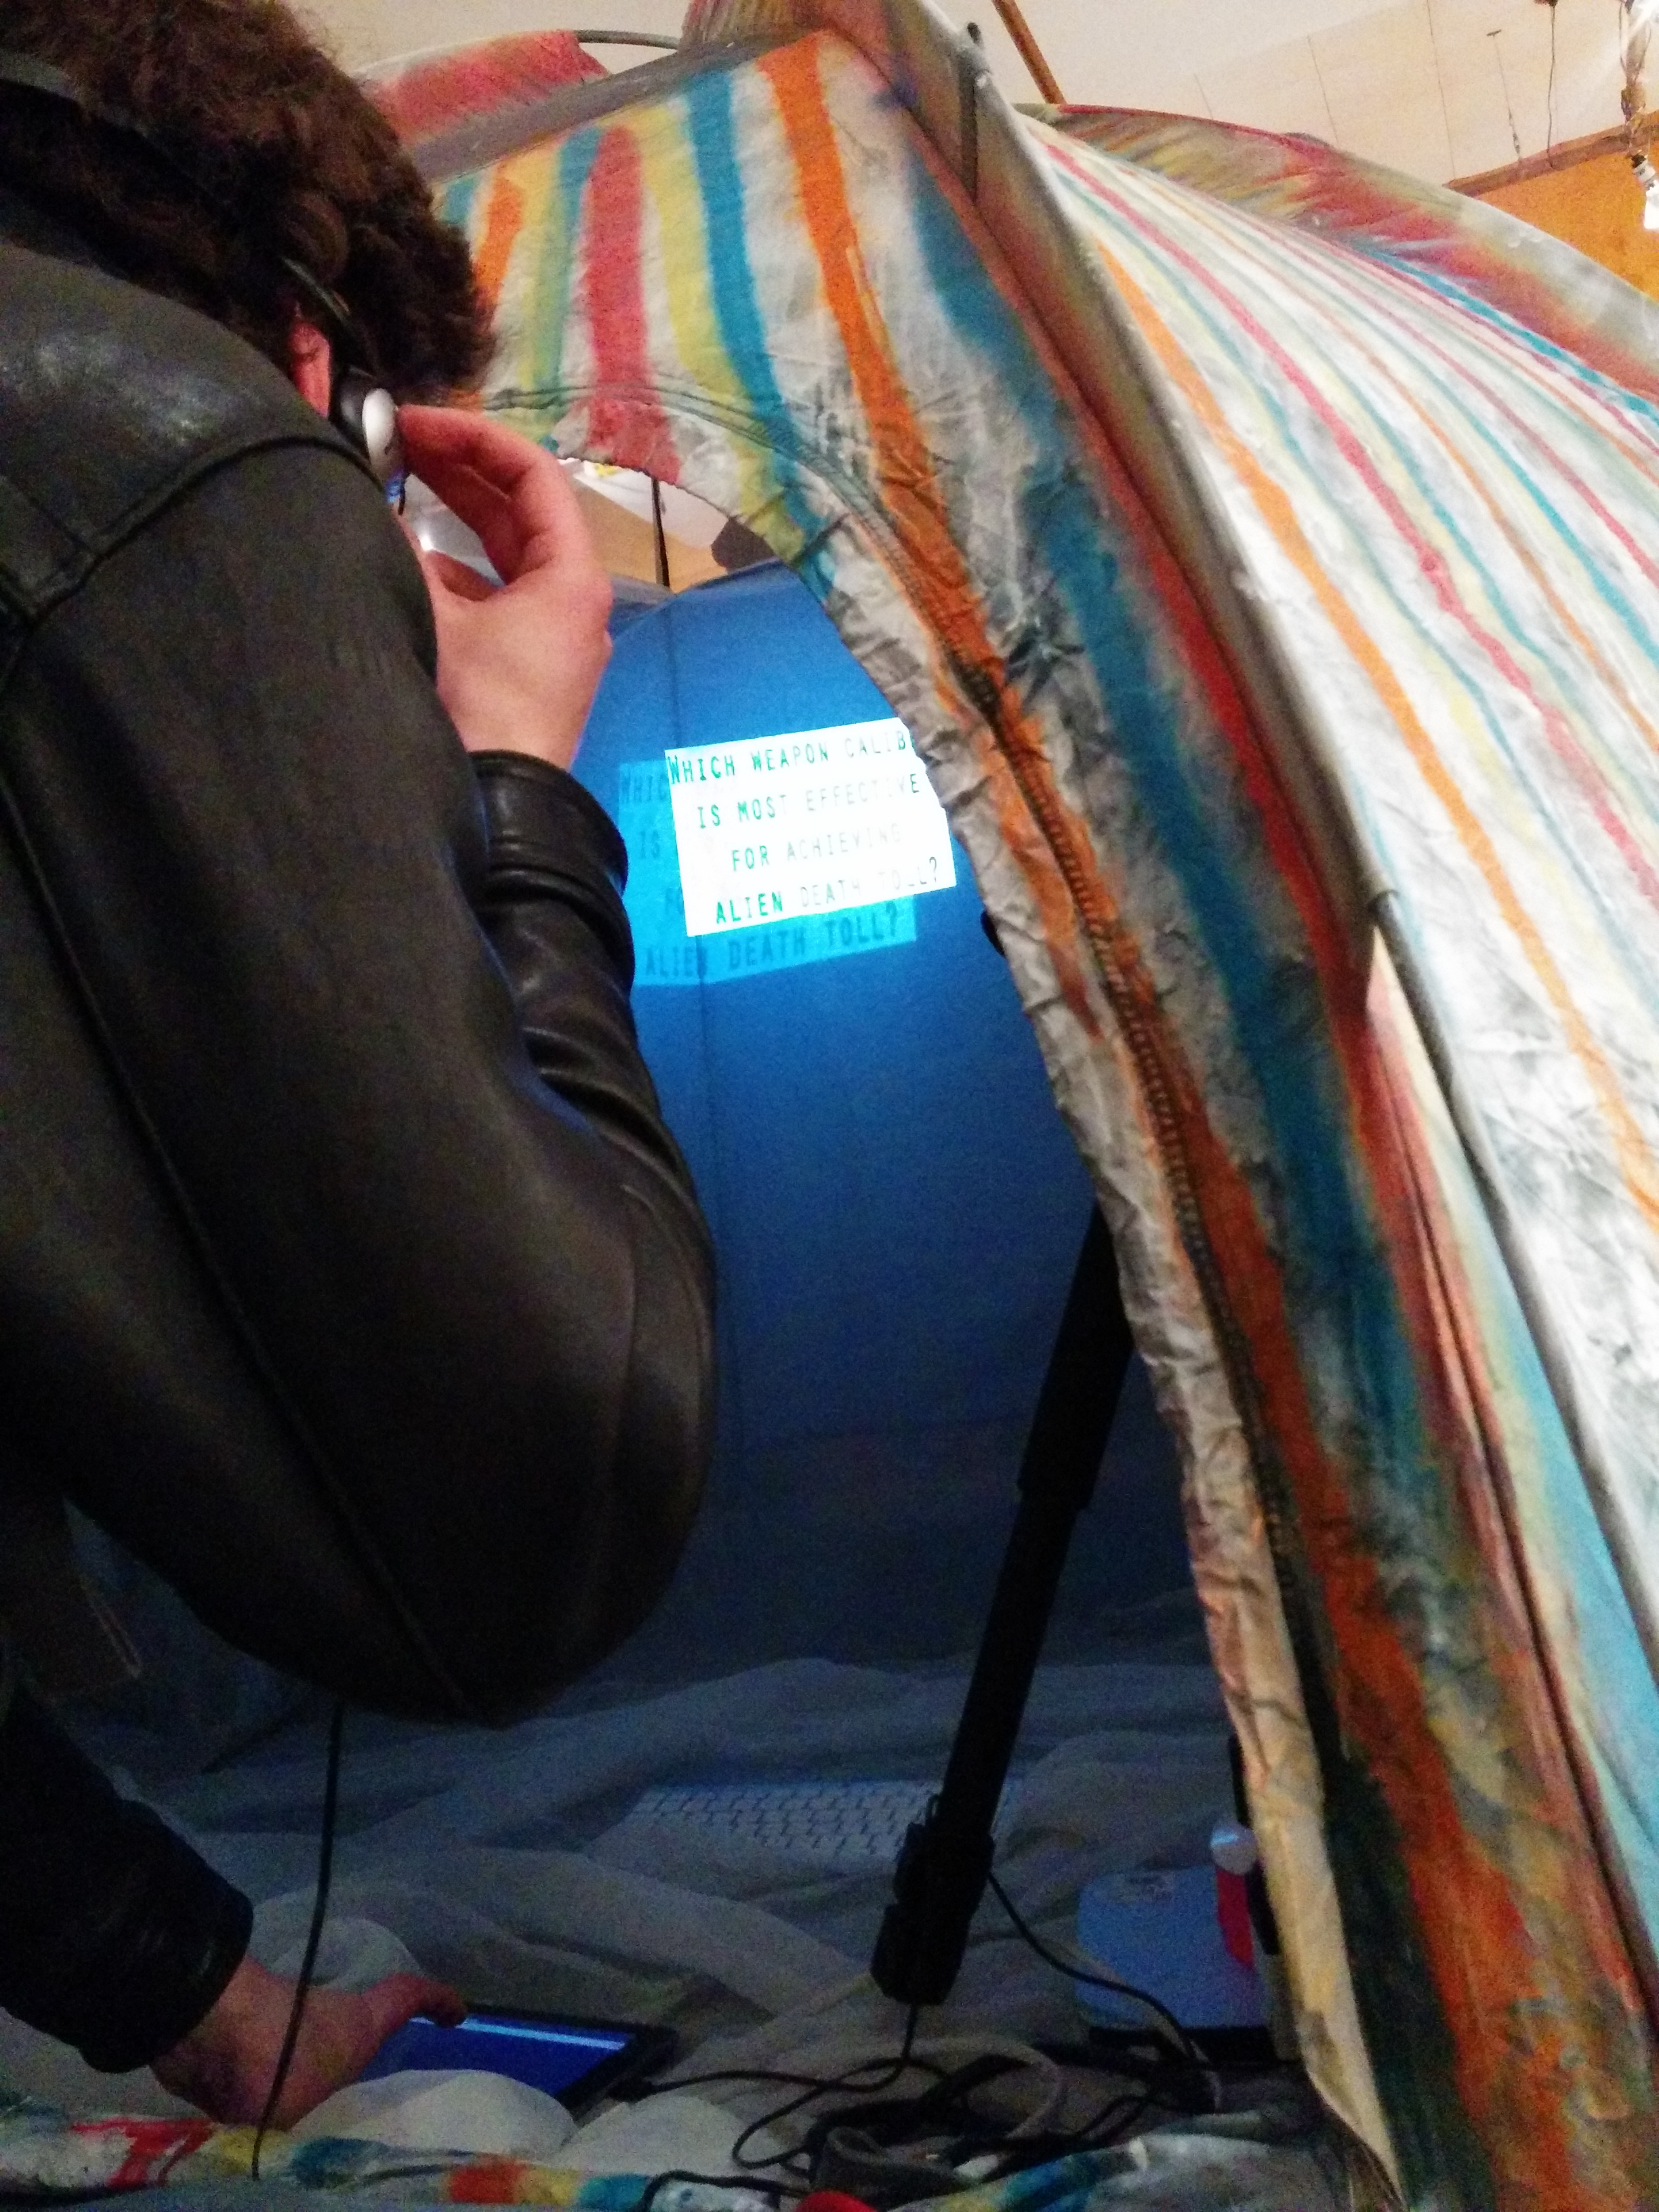
\includegraphics[width=0.7\textwidth]{psXXYborgTentPlay}
  \caption{Hannah Epstein\\\textit{psXXYborg} at FAC 2014, playthrough view}
\end{figure}
\clearpage

\section{Hardware Design}
The success of a project like screenPerfect is dependent not only on its software, or on its ease of use, but on how easy it is to install on-site. The software is dependent on open wifi and high bandwidth to communicate with client devices, a stable computing system, and a variety of computer interfaces. Ideally, the software is open and will work according to standards published by the W3C. In reality, it is incredibly difficult to build a new software system to work on broad platforms.

The following is a list of complications and assumptions built into the design of this hardware, based on public display experiences: 

\begin{enumerate}
\item Data service to an external source cannot be assumed to be available. 
\item The exhibit is assumed to be displayed in public.
\item The environment is assumed to be meterologically hostile - hot or cold, wet or very dry, and to be hosting at least one party, such as an art opening.
\item The exhibition is assumed to be supervised by technically untrained people.
\item The emphasis of the work should be on the work's display, rather than on a laptop screen.
\item The collectors of the work are assumed to have extremely limited resources for rugged workstations.
\item Any host-provided data carriage for external connection - wifi - is assumed to be overloaded by default.
\end{enumerate}

These are all very real constraints that impact display of interactive digital art. We use computers for work and play, but we still separate our lives into periods when we pursue one or the other. There are still boundaries between our personal and public lives. To use the same machines to display art as we do to build the work is to reduce the work from something approachable and consciously displayed to any other tab in a computer. It is my view that digital works especially must be seen within their exhibition context to be understood.

Because the display system needs to be stable and specfic but does not need to be used for development, I began to look into appliance-appropriate hardware. There are a number of low-power ARM-controller based hardware platforms on the market at the time of writing, including the Arduino, the Beagle Bone, and the Raspberry Pi. All of these systems are designed to help artists make interactive works that take advantage of computing power for expression. The Arduino is a popular system for learning to build electronic interactions, the Beagle Bone a full-featured Linux computer, and the Raspberry Pi has come out of an idealistic foundation that hopes to encourage people to learn to program and work with ultra-simplified computing systems.

The Raspberry Pi is my choice for building a hardware installation system to support screenPerfect. The Pi plugs directly into a television set for a monitor, uses Debian Linux for package control, and can store its entire operating system and dependent software on an SD Card - easy to image. Package control means that when one installs software on Debian, the software tends to maintain its own dependencies, which reduces the amount of time a programmer spends adding and removing libraries to get something simple to work. Where an Arduino would require an entire secondary shield to access the internet, the Raspberry Pi is a full computer out of the box, able to access the internet while still being useful from the command line. In addition to this, the computer is the size of a credit card, which makes it straightforward to install in an artistic location such as a van or tent. 

The Raspberry Pi as a platform is also affordable, at \$35 for a Model B with ethernet port and 512Mb of RAM. The Raspberry Pi foundation is a not-for-profit formed to support the opening of technical education to a broad range of children in the UK and overseas. This fit with the ideological stance of game::play Lab and the DMG, as well as my personal politics: that people should be able to use their tools as they see fit. Technology should serve its users, rather than requiring the user to serve technology.

\section{Technical Display Concerns and the Public Private Internet}
screenPerfect's technical display challenges have been embedded in limited systems, such as a reliance on institutional wireless, designed to block filesharing, which also block peer-to-peer experiments such as screenPerfect's server from connecting to its client computers. This resulted in a need for a portable wireless hotspot to serve the application reliably, as in addition to blocking institutional routers, too many users would overwhelm the service. This provided a direction for my primary development to take: the project needed a computer that served both its own web application and provided its own infrastructure, from being turned on to when it was turned off, which did not require any kind of specialized setup for display. In addition, I began to consider how screenPerfect might exist in public space without the requirement of a "smart" screen or any kind of specialized interaction equipment.

People are willing to use their smartphones publicly, but mainly to access the external internet, or messaging services while they are on the move. This led me to consider how people interact with the internet publicly and to consider topics of privacy and public space within the context of how these problems have already been solved by galleries and coffee shops wishing to offer their clientele data services to promote engagement.

In public spaces, internet is supplied by wifi, which comes through a specific type of router known as a "captive portal." A user will walk into a shop, attach to a network, and "sign" an agreement to make use of the wifi within that space. 

Normally, wifi will then give them access to the external internet - the internet as supplied by a major ISP. 
The Raspberry Pi installation of screenPerfect is instead a captive portal, which simultaneously supplies a wifi hotspot and a server that supplies information to that hotspot, without providing external access to the broader internet. This is similar to the pioneering 2013 Eyebeam project \textit{Subnod.es}, in which users pair to a captive portal which is also a server, supplying access to an entirely private chat room, which is available only to users on the network supplied by its own captive portal. 

The first issue addressed by this approach is that there is an inherent contradiction between downloading a site-specific piece to a personal device when the installed context is a core component of the aesthetic experience. Downloading applications to a smartphone seems invasive, particularly if those applications are experimental or site-specific, as I think that screenPerfect games are when they are at their best. The next is that web applications are very much not user-specific - they can be experienced anywhere while they are on the open web, even if their content is intended to be restricted to a specific type of installation, or requires it for best use. By serving the application locally, there is no reliance on an outside pipe. A copy of the game can be sold, customised, and stored in a collection, if such is desired, or installed in any kind of specific cabinet for later use.

\subsection{Subnod.es and Public Private Space}
This project has a precursor using similar technology built at Eyebeam in New York in 2013. Subnod.es uses a captive portal to display a chat client to only the local environment. The differences between screenPerfect and subnod.es are substantial, although mainly located within the code. Subnod.es relies on an external DNS being made available via the actual subnod.es software and depends on a different collection of software to serve the portal proper. It is also built such that those library dependencies are inseparable from the main project script.

The chief concern of subnod.es is that it was built as a response to concerns about communications privacy in North America under the NSA. Specifically, the author of subnod.es is concerned that people behave differently when they are watched, a subset of the concerns generally associated with panoptica and totalitarianism. While I have not specifically structured screenPerfect's Art Portal to address these concerns, it has been built to be largely private. It serves an application to a limited selection of a public space.

The assumption of screenPerfect is that galleries have limited resources but that people who go to art galleries almost certainly have access to a smart phone, which is a form of private space. Smart phones are people's own homes and are built to assume that they will stay with their owners at all times. This means that to install an app is to ask a lot of a viewer: specifically, it is to ask someone to bring an application into their private space without getting to sample it first. In contrast, serving that same application on the broad internet is to entirely delimit the context the art may be experienced within, which reduces its scarcity value to almost nothing while simultaneously removing the curator's ability to set the context of an exhibition experience. This means that it is unlikely an artist can be compensated in any conventional sense despite their large audience. It also means that the curation of the exhibit is no different than the "curation" found on Tumblr.

A better outcome might be to make a limited public space available in a private context. This is what we are doing when we ask that people open their phones and look at a website. The internet is the new public space. By presenting a web application using public technology within the exclusive context of the gallery - or desert, or forest - we take control again over how our art is presented. A gallery or exhibit space can be set up very specifically for the benefit of an audience in a way that the internet in general cannot be. Web technologies are a good solution for this because they are uniform and open in the way that more custom projection design software is not.

This sense of limited private space is key to the code-switching that human communication relies on. We are not the same people in public as we are in private. We are again different people when we are in different publics, from work to the street to school to the gallery. Technology that sensitively addresses these different code contexts seems likely to benefit its authors and users both by permitting the integration of the personal focus with a personal device with the context of a semi-public facility or "safe space" for engagement with the art work.

Safe space is space that has been constructed with an inclusivity policy to promote exploration and community-building within minority groups. It is intended as a systemic resistance to implicit violence. 

\section{Distribution of Work}
An optimal route to distribute both screenPerfect and the works produced with the tool is to compile them on an SD Card using the node-webkit package, which permits the distribution of web applications as desktop software without losing the multi-device communication channels supplied by a webserver. This could then be distributed digitally over the internet.

Futher, screenPerfect has already been forked. The system is publicly available on Github to permit anyone to extend the software. The Node.JS package can be compiled to include Windows, Linux, and OSX distributions, as well as being installed directly to a Raspbian - Raspberry Pi Debian - operating system, which would then launch the game or tools on boot. 

 

% Chapter Template
% Chapter Template
\setstretch{1}
\chapter{Conclusion}\thispagestyle{empty} % Main chapter title

\label{Chapter5} % Change X to a consecutive number; for referencing this chapter elsewhere, use \ref{ChapterX}

\lhead{Chapter 5. \emph{Conclusion}} % Change X to a consecutive number; this is for the header on each page - perhaps a shortened title
\setstretch{2}
%----------------------------------------------------------------------------------------
%	SECTION 1
%----------------------------------------------------------------------------------------

\section{Conclusion}

Artist-led research results in an exploration of not only what is considered popularly reasonable but also what is possible. By anchoring that practice to community feedback from a group of invested users, we can expand software from beyond its original audience to a new section of the population and then work through the specific display and installation requirements for that group. By making the software with a specific user in mind, we both ensure demand and reward involvement with the work; by committing to that work as "real," we can produce new directions for design. Demand here is constructed not as capitalist \textit{massive} or unlimited demand but instead the niche requirements indicated by the new, broader, connected public space. It is possible to have a small overall demand be, in aggregate, worthwhile.

screenPerfect has already been forked into new tools to work towards the likelihood that gamemakers will pursue new video works. Bento Box-Miso's iV fork, which discards dual-screens but encourages branched FMV narratives to be pursued within DMG, was launched at Feb Fatale 2 in early 2014 and has seen some popular uptake. This is an important marker of the overall success of this embedded research. A possible direction for this software is to package it so that games built with it can be installed both locally and remote at the same time in public contexts. The installation of those games in public contexts will be supported by further work on hardware systems for easy, portable, open hardware, that can then be reliably exhibited in new contexts. Distribution of the completed work can take place over the internet as a pre-configured operating system, which, similar to a game cartridge, means that users and gallery specialists need only do a minimum of support work to install, repair, replace and update digital works produced with this system. In addition, this software can be stored on SD cards with backup Raspberry Pi, ready for installation for an indeterminate period of time into the future.

In Cixous' "Laugh of the Medusa" \parencite{cixous} she states that to be considered real, women must write for themselves. This document extends the notion of the written self to the world of code, and through it to computers and the contemporary technological landscape: one must write after one's own interests in order to represent a possibility for what one believes can be real. I have done this by writing a tool that permits an array of interested parties to produce games without a reliance on conventional scripting or game assets. I have then extended screenPerfect with hardware to support a straightforward installation path using materials from a not-for-profit foundation and open-source software, rather than a limited system reliant on strictly commercial ties.

This prototype emphasises allowing an audience to experience digital works as easily as possible in a context controlled by the artist. Works produced using screenPerfect can be displayed anywhere a series of screens and a single server can be set up. This emphasis on experience moves the interaction sphere of art and gaming into the world. screenPerfect's impact is most felt at night, outdoors, or in temporary installations. However, using screenPerfect, it is possible to display video-art and collaborative gameplay anywhere at all. These are the new/old/new exhibits, the one-time-only parties, the experience that happens in a hard to access place yet leaves no marks for future visitors to interpret, such as Nuit Blanche in Toronto, or Burning Man in Nevada. At the heart of screenPerfect is the idea that we can pull away from artificial distance and have instead on-site participation, unique experiences that project real, contemporary art into real, contemporary spaces.

Throughout the development of screenPerfect, I asked a series of questions about capital, monetary and otherwise, creative practice, and preservation in the digital context. This is an effort to directly address the debate about games as art by circumventing it: as we can see by visiting Cixous, any form of creative practice can be dismissed by the dominant voice. A debate about whether a given creative practice is worthy of the name "art" is in fact a form of access control. By testing a piece of software developed through one artist's working practices with a broader audience, we can add resilience to the code. This helps to ensure that it serves both the intended process and supports further experiments. This permits broad access to expression on behalf of new voices while simultaneously stress-testing the work itself. By giving people open tools, we give them the ability to express themselves: if what they would like to say is then something personal, it is my view that there is value in that.

We live within a system of value and valuation. To overcome all elements of that system from within is unlikely - an assertion supported by mathematicians like Gödel as much as feminists like Audrey Lorde - but we do not need to overcome the system to be able to circumvent it. We can choose how much to engage with the system, on what terms. Within that effort we may find answers to specific problems.
 
% Chapter Template

\chapter{Endnotes, References, Works Cited} % Main chapter title

\label{Chapter6} % Change X to a consecutive number; for referencing this chapter elsewhere, use \ref{ChapterX}

\lhead{Chapter 6. \emph{Endnotes, References, Works Cited}} % Change X to a consecutive number; this is for the header on each page - perhaps a shortened title

%----------------------------------------------------------------------------------------
%	Works Cited
%----------------------------------------------------------------------------------------

\section{Works Cited}


Anna Anthropy, Rise of the Videogame Zinesters, http://www.auntiepixelante.com/games/
Merrit Kopas, http://mkopas.net/
Zoe Quinn, http://www.beesgo.biz/
Zach Blas, http://www.queertechnologies.info/products/gay-bombs/
Porpentine, http://aliendovecote.com/
Soha El-Sabaawi, http://www.el-sabaawi.com/

\subsection{Software}
 
% Chapter Template

\chapter{Endnotes, References, Works Cited} % Main chapter title

\label{Chapter7} % Change X to a consecutive number; for referencing this chapter elsewhere, use \ref{ChapterX}

\lhead{Chapter 7. \emph{Endnotes, References, Works Cited}} % Change X to a consecutive number; this is for the header on each page - perhaps a shortened title

%----------------------------------------------------------------------------------------
%	Works Cited
%----------------------------------------------------------------------------------------

\section{Works Cited}


Anna Anthropy, Rise of the Videogame Zinesters, http://www.auntiepixelante.com/games/
Merrit Kopas, http://mkopas.net/
Zoe Quinn, http://www.beesgo.biz/
Zach Blas, http://www.queertechnologies.info/products/gay-bombs/
Porpentine, http://aliendovecote.com/
Soha El-Sabaawi, http://www.el-sabaawi.com/

\subsection{Software}
 

%----------------------------------------------------------------------------------------
%	THESIS CONTENT - APPENDICES
%----------------------------------------------------------------------------------------

\addtocontents{toc}{\vspace{2em}} % Add a gap in the Contents, for aesthetics

\appendix % Cue to tell LaTeX that the following 'chapters' are Appendices

% Include the appendices of the thesis as separate files from the Appendices folder
% Uncomment the lines as you write the Appendices

% Appendix A
\setstretch{1}
\chapter{screenPerfect Installation Guide} % Main appendix title

\label{AppendixA} % Change X to a consecutive letter; for referencing this appendix elsewhere, use \ref{AppendixX}

\section{screenPerfect Code and Documentation}
The code of screenPerfect is located on the DVD included in this volume, and at \url{http://www.github.com/pretentiousgit/screenperfect-dev}. This DVD includes five games produced for the screenPerfect Engine: PornGame, psXXYborg, OM, Grimoire, and Cyborg Goddess.

\section{Device List}

\begin{enumerate}
\item{Large powerbar with surge protection and power supply cable}
\item{Server with Node.JS installed}
\item{Projector or monitor}
\item{Portable wireless hotspot}
\item{Touchscreen device with browser software}
\item{Optional: Speakers with subwoofer}
\item{keyboard}
\item{mouse}
\item{power supply}
\item{hdmi or vga cables as appropriate}
\end{enumerate}

\section{Software List}
\begin{enumerate}
\item{Google Chrome (preferred), on all devices likely to play.}
\item{screenPerfect will also run on Safari, but there are issues due to Google’s refusal to support the MP4/h.264 video codec (large, but good quality) and Apple’s similar refusal to support V8/webM (small, better, owned by Google).}
\item{NodeJS installed on screenPerfect’s host computer.}
\item{git installed on screenPerfect’s host computer.}
\item{Miro VideoConverter on a mac system}
\end{enumerate}

\section{Installation and Site Construction}

\subsection{Before Leaving For Site}
\begin{enumerate}
\item{Ensure NodeJS is installed and functional on main server.}
\item{Install latest repository of screenPerfect from GitHub.}
\item{Ensure all video files are present and accounted for in all appropriate formats.}
	\begin{enumerate}
		\item{webM}
		\item{MP4}
	\end{enumerate}
\item{Find surface to project on.}
\item{Lay out power cable and power bar.}
	\begin{enumerate}
		\item{power to wireless hotspot}
		\item{power to main server}
		\item{power to projector}
		\item{power to support tablet interface}
		\item{power to speakers}
		\item{monitor/projector}
		\item{keyboard}
		\item{mouse}
	\end{enumerate}
\item{Connect devices to their relevant power supplies.}
\item{Plug in green jack of speakers to headphone jack of main server.}
\item{Turn on all devices.}
\item{Turn off all mobile data for wireless hotspot device. If necessary, remove SIM.}
\item{Turn on wireless hotspot.}
\item{Turn on your main server.}
\item{Connect to your wireless hotspot.}
\item{Open Terminal (Mac), navigate to screenPerfect’s home directory, turn on screenPerfect}
	\begin{enumerate}
	\item{Navigate to the game folder you wish to run by typing "cd" and then the directory path at the prompt.}
	\item{type node screenPerfect, press enter.}
	\item{You will see a message saying “screenPerfect listening on port 3003”.}
	\end{enumerate}
\item{Open a new tab in Terminal (command-T)}
\item{Type ifconfig to get the IP address of your wireless hotspot.}
\begin{enumerate}
\item{look for the value called "inet" - it will be a \url{192.168.x.x} address if you are attached to the hotspot, and (probably) \url{10.x.x.x} if you’re attached to a wider network.}
\end{enumerate}
\item{On the Server, Open Chrome and navigate to \url{http://0.0.0.0:3003/client}}
\item{Open Terminal, and in the tab where you typed “node screenPerfect”  there will be a stream of messages about a heatbeat.}
\item{There should also be a video playing in your browser now.}
\item{On the Tablet Device, open Chrome. Replace the below values with the ip address located in step 14a}
\begin{enumerate}
\item{\url{http://x.x.x.x:3003/control}}
\end{enumerate}
\item{If all goes well, the “Start” button will appear onscreen on your tablet.}
\item{Touch the start button, and the projected video will change.}
\end{enumerate}

\section{Troubleshooting}

\subsection{On Start, Google Chrome Cannot Find Control Screen}

\begin{enumerate}
	\item{Check that the Tablet is on the wireless network provided by the hotspot.}
	\item{If not, repair the hotspot by disabling it, reenabling it, and reconnecting both the server and the tablet to the same network.}
\end{enumerate}

\subsection{The Control Device is frozen, or the videos are not changing.} 

Just about anything else, really, including the above.
\begin{enumerate}
	\item{Open the Terminal.}
	\item{Check the heartbeat stream for an error such as “Abort Trap,” “Bus Trap,” or “stream error in pipe.”}
	\begin{enumerate}
	\item{All of these are normal. They are a result of someone tapping the screen quickly enough to overwhelm the server.}
	\end{enumerate}
	\item{type node screenPerfect and press enter to restart the application.}
	\item{Refresh the tablet browser and press the start graphic to make sure the video is being served.}
	\item{Refresh the server browser to ensure everything is passed correctly.}
\end{enumerate}

\section{Tidbits and Tech Notes}

\begin{itemize}
	\item{People with little technical experience will sometimes have trouble determining if they have actually touched/interacted with the app appropriately. Some may accidentally exit the application on the tablet, and may be unsure of how to re-enter the experience.}
	\item{screenPerfect is most rewarding when played in isolated concentration somewhere quiet. It is challenging to concentrate on the video enough to get full effect if people are distracted.} 
	\item{screenPerfect crashes approximately once per three hours of play time, more in high temperatures.}
	\item{screenPerfect games work best in Android, as Android supports the webM/V8 codec. Apple devices require mp4s, which are approximately 4x the size.}
	\item{screenPerfect was developed in JavaScript using ExpressJS for NodeJS. screenPerfect was developed on a MacBook Pro for use with Chrome, but will function almost as well with Safari.}
\end{itemize}
% Appendix Template

\chapter{Game Jam Documentation} % Main appendix title

\label{AppendixB} % Change X to a consecutive letter; for referencing this appendix elsewhere, use \ref{AppendixX}

\lhead{Appendix B. \emph{Game Jam Documentation}} % Change X to a consecutive letter; this is for the header on each page - perhaps a shortened title

%----------------------------------------------------------------------------------------
%	Initial Questions
%----------------------------------------------------------------------------------------

\section{Interview Files}
Interview sound files can be found on the Supporting Materials DVD within the "Game Jam Interviews" folder.

\section{Questions To Ask Game Jammers}


\begin{itemize} 
\item[\tiny{$\blacksquare$}] What were you expecting when you came to the jam?
\item[\tiny{$\blacksquare$}] What features did you immediately want in your software?
\item[\tiny{$\blacksquare$}] How has your group process worked throughout the week?
\item[\tiny{$\blacksquare$}] How is your group process going today?
\end{itemize}

\subsection{Games List}
\begin{itemize} 
\item[\tiny{$\blacksquare$}] Porn Game by Maxwell Lander
\item[\tiny{$\blacksquare$}] Grimoire by Katie Foster and Mikayla Carson
\item[\tiny{$\blacksquare$}] Kill Fuck Marry by 
\item[\tiny{$\blacksquare$}] Mind Safe by Dann Toliver and Robby
\item[\tiny{$\blacksquare$}] Glitch95 by Arielle, Rebecca and Bronwyn
\item[\tiny{$\blacksquare$}] Omm by Brittany and Diana
\item[\tiny{$\blacksquare$}] Cyborg Goddess by Cara and Kate McKnyte
\item[\tiny{$\blacksquare$}] Empty Puppet by Danielle Hopkins and Dawn
\end{itemize}

\subsection{Bug Discovery}
\begin{itemize} 
\item[\tiny{$\blacksquare$}] Room Zero must be the first room edited.
\item[\tiny{$\blacksquare$}] Room Order cannot be altered in a meaningful way - ID is hidden from users
\item[\tiny{$\blacksquare$}] WebM video is unplayable on Apple devices
\item[\tiny{$\blacksquare$}] H.264 video is slow to unplayable on non-Apple devices
\end{itemize}


%----------------------------------------------------------------------------------------
%	Raw Notes
%----------------------------------------------------------------------------------------
\subsection{Features Requested by Game Jammers}

\begin{itemize} 
\item[\tiny{$\blacksquare$}] Sound effects on control input - requested by Arielle
\item[\tiny{$\blacksquare$}] Timed hotspots which appear and disappear on specific video cues
\item[\tiny{$\blacksquare$}] A game tracer that tracks which choices players make, and records their games
\item[\tiny{$\blacksquare$}] Gesture controls - pinch, zoom, throw - on touchpoints.
\item[\tiny{$\blacksquare$}] Tree View to visualize how a game is laid out
\item[\tiny{$\blacksquare$}] Rooms cannot be deleted - delete and reorder rooms
\item[\tiny{$\blacksquare$}] Games cannot be deleted - delete and reorder games
\item[\tiny{$\blacksquare$}] Copy and paste room layouts so that one does not have to recreate grids - done.
\item[\tiny{$\blacksquare$}] Hotspots that can move around the room.
\end{itemize}

\subsection{Notes from committed jammers about screenPerfect}

For Arielle, the most engaged of the jammers, the idea of turning any touch device into a custom console controller, with custom buttons, is engaging. The more traditional the game developer, the harder a time they had with the idea that they'd be showcasing content with the narrowest help from the new tool. The filmmakers were very impressed with the ability to not touch a darn thing and have considerable success.

% Appendix Template

\chapter{Raspberry Pi Setup Documentation} % Main appendix title

\label{AppendixC} % Change X to a consecutive letter; for referencing this appendix elsewhere, use \ref{AppendixX}

\lhead{Appendix C. \emph{Raspberry Pi Setup Documentation}}

 
\section{Materials and Supplies}
\textbf{Raspberry Pi}
The Raspberry Pi is a full linux computer the size of a large credit card. A Raspi runs Debian linux off of a common SD card.
\textbf{32Gb SD Card for Raspberry Pi}
This is where we place the operating system and software for the Pi.
\textbf{USB wiFi dongle}
Edimax-based wiFi USB dongle, for serving wiFi hotspot on the Pi.
\textbf{USB flash memory}
For transferring or storing complete programs authored on external systems.
\textbf{Keyboard and Mouse}
For initial computer setup.
\textbf{Ethernet Cable}
Standard cat5 ethernet cable for programming remote.
\textbf{HDMI TV and cable}
Used as a monitor for the Raspberry Pi.
\textbf{Micro USB and power supply}
Power for the pi.
\textbf{Mac or PC computer with USB ports, ethernet port, SD Card reader}
Required for raspberry pi setup.

\section{Background for Linux Commands}
sudo means "do this now even if I appear to have insufficient user permissions" in Linux 
apt-get is an inherited "package manager" from Debian linux. "Dependencies" are the software your software requires to run, Debian uses apt-get to manage them.
Things that follow sudo are commands.

\section{Setting Up The Raspberry Pi}
\subsection{Windows 7 SD Card setup and first boot}
This section is written for a Windows 7 environment, and is based on the common tutorial at \url{http://learn.adafruit.com/adafruit-raspberry-pi-lesson-1-preparing-and-sd-card}
\begin{enumerate}
\item Connect your main computer to the internet.
\item Download the most recent Raspbian distribution image from \url{http://www.raspberrypi.org/down}
\item Download Win32DiskImager from the greater internet. This is preferable because it allows you to write image backups to your harddrive.
\item Using Win32DiskImager, write your Raspbian distro to your SD card on your main computer.
\item Eject the microSD card and stick it into the Raspberry Pi.
\item Plug in your keyboard, and plug a mouse into your keyboard.
\item Plug in your HDMI cable and monitor. Turn them on.
\item Plug in the MicroUSB cable for power to the Raspberry Pi.
\end{enumerate}


\subsection{Configuring Raspbian}
Once the RasPi is turning on, it needs to be set up to include all of its software. Turn the Pi on, and wait until the blue configuration screen comes up.
Figure 4.3: Early RasPi Configuration Screen

\begin{enumerate}
\item expandrootfs Expand the boot system so that you will not run out of onboard memory for software.
\item memorysplit Reduce the GPU to minimum, because we will be using the raspi as a headless server from the command line.
\item changepass Change the password so that the Raspberry Pi will be less easy to hack.
\item ssh Enable SSH so that the pi will be accessible from an external computer.
\end{enumerate}

When done, select finish to exit.
Type sudo reboot to restart the raspi.

\section{Software Setup for External WiFi Access}
A wiFi antennae can be used for one purpose at a time: it can either be used to access the external internet, for acquiring software to install into the raspi, or it can be used for serving a hotspot. It cannot do both at the same time. To load the pi up requires external access, so we will be loading that first. You must configure your wiFi before plugging in your wiFi antenna. 

In Linux, there is warning you if you mistype a folder name, say, adding an "s" to "network" to make it "networks." If you would like to confirm your folder name is correct, try typing "ls /etc/" to list the contents of that directory. Network is a default folder, and Interfaces is already present at first boot, so you can make sure your things are all there before you really get started. The way to tell you have done something wrong is if you type the below command and an empty new file opens. You are editing a file here, not creating one.
 At your console prompt, type the following:

\begin{lstlisting}
sudo nano /etc/network/interfaces
\end{lstlisting}

This opens a text editor called 'nano.' Enter the following into it.
\begin{lstlisting}
auto lo

iface lo inet loopback
iface eth0 inet dhcp

allow-hotplug wlan0
auto wlan0

iface wlan0 inet dhcp
wpa-ssid "network name, commonly called an ssid, goes here"
wpa-psk "password"
\end{lstlisting}

Then type CTRL-X and Y to save your file.

\begin{lstlisting}
sudo halt
\end{lstlisting}

Plug in your wifi antennae, pull the Raspberry Pi's power cable, and plug it back in. This should make the raspi's antennae turn blue as it turns on. This little blue LED will frequently be the only way to tell something is going correctly or incorrectly, so it is an excellent tell that your machine is running.

Plug in your wifi antennae, pull the Raspberry Pi's power cable, and plug it back in. This should make the raspi's antennae turn blue as it turns on. This little blue LED will frequently be the only way to tell something is going correctly or incorrectly, so it is an excellent tell that your machine is running. 

The case in the following figures is a modification of an open-source design supplied by Thingiverse.com user DrewTM. It is Thing \#114244 and can be found at https://www.thingiverse.com/thing:114244.

\newpage
\begin{figure}[h!]
 \caption{Raspberry Pi with functioning wiFi antenna}
 \centering
  \includegraphics[width=0.5\textwidth]{raspiWiFi}
\end{figure}

\begin{figure}[h!]
 \caption{Raspberry Pi in Thingiverse case}
 \centering
  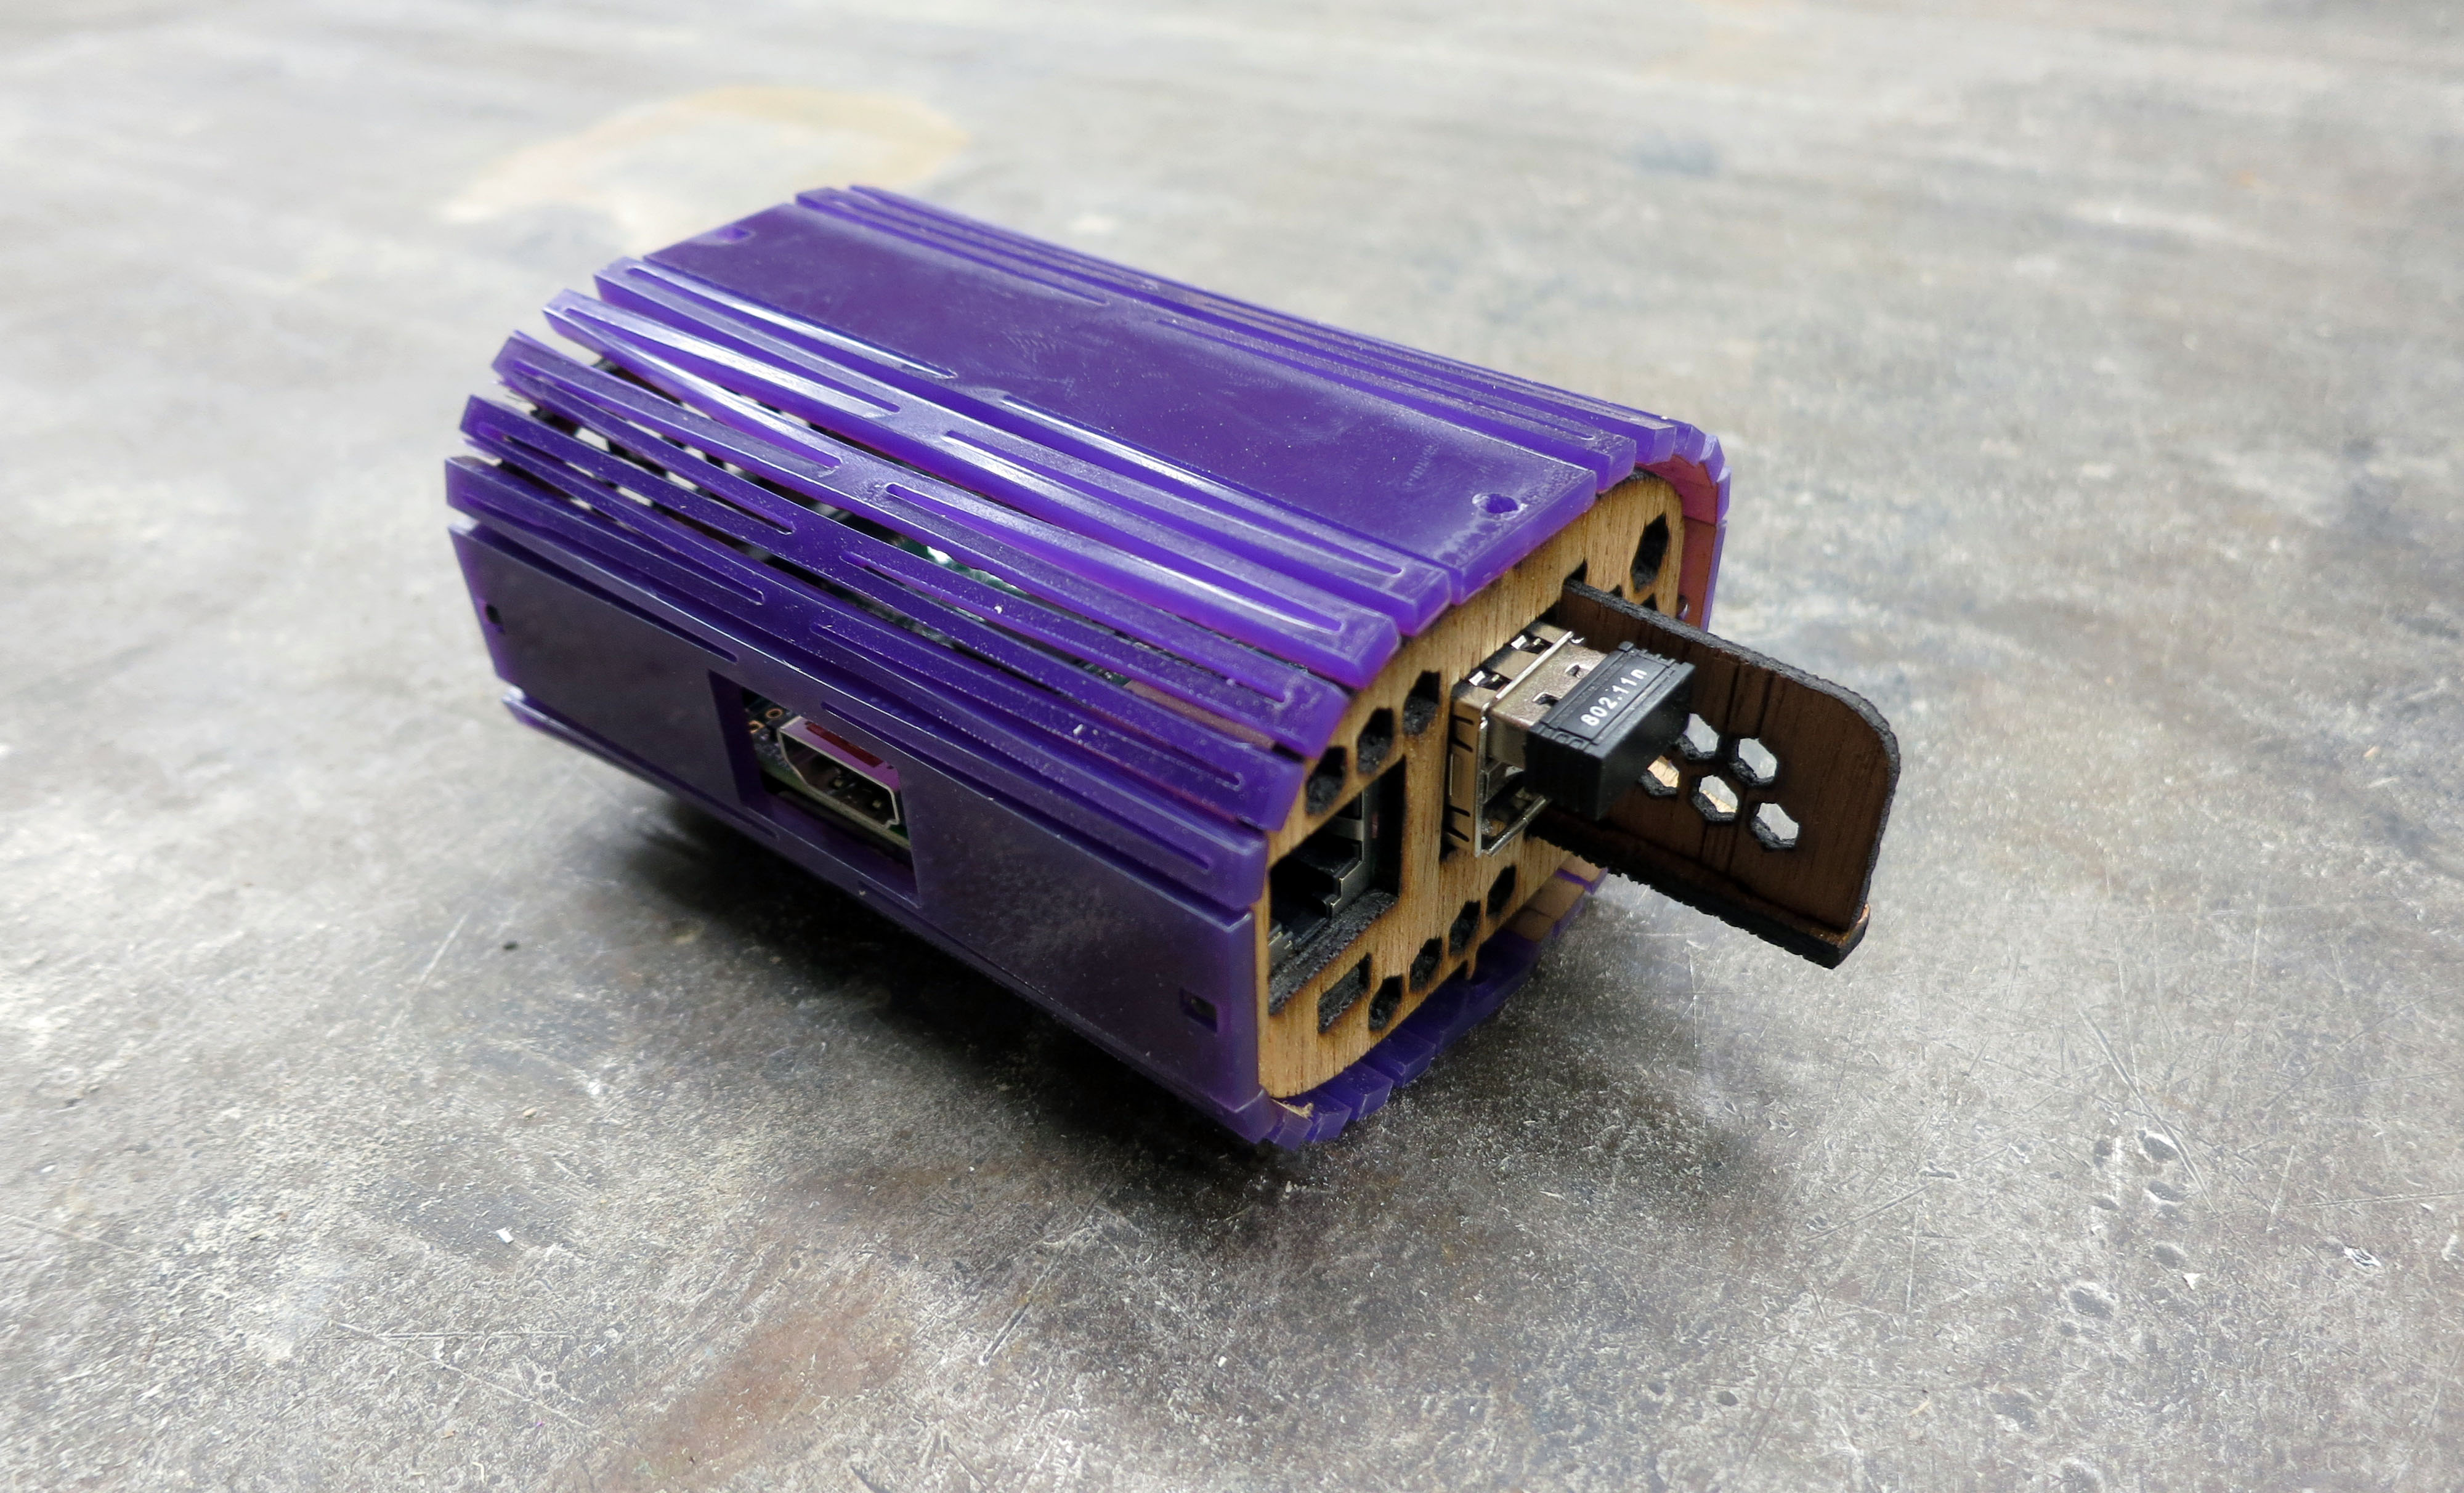
\includegraphics[width=0.5\textwidth]{raspiCase}
\end{figure}

\newpage

If all went well, you've now connected to your own supply of wireless internet. This will not work if you are using an 802.1x network, such as those within OCADu. On your own home network, however, type:

\begin{lstlisting}
sudo apt-get upgrade; sudo apt-get update
\end{lstlisting}

This will upgrade your rasppi to whatever the latest agreed-upon package lists are, then update those packages to their most recent approved version.

\section{Installing Node.JS}
\subsection{Why Node?}
I've chosen to install Node because it is the software framework I selected to run the new game engine built in Part 1 of this thesis. Node is a new framework designed to get Javascript running on a server. There are advantages and disadvantages to this approach. The advantages are that JavaScript is a beautiful, minimal language that is relatively easy to learn. The disadvantages are that there is a heavy public bias against JS due to its years as a client-only language designed to manipulate what are known as Document Object Model (DOM) elements in-browser.

The brilliance of Node is that it replaces the need for a specific input-output window, replacing that definition requirement with any internet browser. Node, backed by Google's V8 engine, currently works best on Chrome, but it can interact with any browser.

Node is therefore easy to use, and easy to program for from the perspective of a mainly web based development chain. 

\subsection{Installation Instructions for Node.JS}
Create a directory for Node to live in by typing the following at prompt.
\begin{lstlisting}
sudo mkdir /opt/node
\end{lstlisting}

Acquire the node "tarball" - compressed framework files - via the internet.

\begin{lstlisting}
wget http://nodejs.org/dist/v0.10.2/node-v0.10.2-linux-arm-pi.tar.gz
\end{lstlisting}

Unzip (desticky from tarball) it:
\begin{lstlisting}
tar xvzf node-v0.10.2-linux-arm-pi.tar.gz
\end{lstlisting}

Copy the contents of the newly unzipped folder and paste them to your new directory. This leaves a copy of the tar and a copy of the unzipped tar at their original locations. You can probably remove them using sudo rm when you're sure everything is where it should be.

\begin{lstlisting}
sudo cp -r node-v0.10.2-linux-arm-pi/* /opt/node
\end{lstlisting}

Edit - or create - a .bash_profile file, which is a type of script that runs when you turn on the pi. In this case, it runs and tells Node that it exists on your computer, so that typing node runthisprogram will do something. What is a .bash_profile?

From your root directory, to open a new nano text file:
\begin{lstlisting}
sudo nano .bash_profile 
\end{lstlisting}

Then add the following and save it to your new .bash_profile file...

\begin{lstlisting}
PATH=$PATH:/opt/node/bin 
export PATH
\end{lstlisting}

Control-X, Y to save it.

Node lives in the \texttt{/opt/node} directory you created above. This adds the commands "node" and "npm" to what are called "environment variables." If you are curious, and god knows you must be to play with a raspi, you can type \texttt{ls /opt/node/bin} and see the little programs sitting there in their bin.

\section{Testing Node}
Node will need to be able to fetch its own packages separately from the raspi from the internet in order to run some of the monitoring software I've chosen to use. Particularly, you will need the \texttt{forever} package.

\subsection{Selecting Monitoring Software}
\texttt{forever} has ultimately been the software I've decided on to monitor and run screenPerfect, because it is a node-native package that keeps things running even when they crash. There are other software packages used for broader deployment, such as Monit, which installs to your Debian parcel rather than to Node. Monit typically runs with what is called an HTTP Proxy, which can be written directly in Node or installed independently. In a full deployment build, Monit and HAProxy would be preferable to Node alone, because this follows the best practice of separating out different programming elements from one another in production. Monit and HAProxy can also deploy applications above and beyond Node itself, which is preferable for things written in Python, for example. 

For this example, though, \texttt{forever} works well. It provides monitoring to tell us what the application is doing, and automatically restarts node applications when they crash. Were I deploying this such that it could keep an eye on the internet, which I am not, I would also include \texttt{nodemon}, as is recommended by the Subnod.es project. \texttt{nodemon} monitors your development code and pushes changes from a central server to your deployment automatically.

That is outside the scope of this paper at present. 

\subsection{Installation of Node Modules}
To install a node package - or "module" - you type 

\begin{lstlisting}
npm install PACKAGENAME
\end{lstlisting}

To install one globally, type
\begin{lstlisting}
npm install PACKAGENAME -g
\end{lstlisting}


To absolutely force install:
\begin{lstlisting}
sudo su
PATH=/opt/node/bin/:$PATH
npm install PACKAGENAME -g
exit
\end{lstlisting}

To install \texttt{forever} and \texttt{nodemon}
\begin{lstlisting}
npm install forever -g
npm install nodemon -g
\end{lstlisting}

To run \texttt{forever} and \texttt{nodemon} together....
\begin{lstlisting}
forever start /usr/local/bin/nodemon /path/to/YOURAPP.js
\end{lstlisting}

\subsection{Troubleshooting NPM installations}
When I tried to install \texttt{forever} the first five times, it timed out, gave me a 404 error repeatedly, and declared I had insufficient permissions to do a global install. This is where computer science faith, confidence, and patience come in. When the install did not work for half an hour, I took a break, came back, and discovered that it installed the next day.

This process is heavily dependent on a massive network of computers and other people. In development, it is quite likely things beyond one's own control are going to go wrong. Going for a break will help you keep patient.

\section{SSH via Direct Ethernet Connection\\ and WiFi Internet Access}
Eventually, you will need both of the powered USB slots on the raspi for a USB key and for your wiFi. In addition, the raspi doesn't have the power to drive a monitor and consistently serve wiFi out of its USB ports. To get around this, it is most convenient to be able to SSH in to your device. Although it appears to be best practice to use the wpa_supplicant file to store how you wish the Raspberry Pi to connect to the internet, I have had limited success with it, likely because I am not configuring a static IP for my raspi properly.

My \texttt{/etc/network/interfaces} file looks like this:
\begin{lstlisting}
auto lo
iface lo inet loopback

auto eth0
iface eth0 inet static
address [MY MAIN TERMINAL'S ETHERNET IP PLUS ONE]

auto wlan0
allow-hotplug wlan0
iface wlan0 inet dhcp
   wpa-ssid "network name here"
   wpa-psk "dubiously secure password"
\end{lstlisting}
 

\begin{lstlisting}
sudo nano /etc/default/ifplugd

### MANY TALK, HOW COMMENT, SUCH WARNING ###
INTERFACES="eth0"
HOTPLUG_INTERFACES="eth0"
ARGS="-q -f -u0 -d10 -w -I"

SUSPEND_ACTION="stop"
\end{lstlisting}

This is an edit of the existing bits, and I can't tell if it will break everything long-term.
Here is what your startup script should read. This ensures that your wiFi antenna turns on, which is likely not something it was doing when you plugged in your ethernet directly.

\begin{lstlisting}
sudo nano /etc/rc.local
#!/bin/sh -e

# Print the IP address
_IP=$(hostname -I) || true
if [ "$_IP" ]; then
 printf "My IP address is %s\n" "$_IP"
fi

# Disable the ifplugd eth0
sudo ifplugd eth0 --kill
sudo ifup wlan0

exit 0
\end{lstlisting}

CTRL-X and Y to save, then \texttt{sudo reboot} open a terminal on your main laptop. On your laptop, at the prompt, enter:
\begin{lstlisting}
ssh pi@[the static ip address you entered under eth0 static above]
\end{lstlisting}

Your \texttt{pi@[static ip]} should appear in your terminal window, which means you can now talk to raspi.
Per usual, to ensure your wifi is still working properly, try a \texttt{sudo apt-get update} or \texttt{ping google.com}, both should return you data.

\section{Backing Up the Raspberry Pi}

Now that everything has been configured for the first steps, type \texttt{sudo halt}, and when the Raspberry Pi turns off, remove the SD card from it. Place the SD card back in your main computer and reboot Win32DiskImager.

Create a new file folder somewhere within your Documents folder. I called mine Raspberry Pi Backups.

In the Write From section of the application, select your SD card, which is probably called boot. In the Write To section, select your new folder. 

Write a copy of the kernel image from the boot card to the new backup directory. Then safely eject your SD Card and re-insert it in the RasPi. It is best practice to form these occasional backups as you proceed through set up. Many of these steps can cause the Raspberry Pi distro to break badly. A backup will save a great deal of time when the inevitable happens.

\section{Mount Your USB Flash Memory Stick To the Raspberry Pi}

\subsection{Configuring Your Mount Drive}
This bears some thinking about, because the \texttt{/media/} folder is for media, and you are instead choosing to run a program off of the drive. Subnod.es suggests making it your \texttt{www} drive, for world wide web. I picked \texttt{/mnt/}.

Find your USB memory by listing the the things plugged into dev:
\begin{lstlisting}
sudo ls /dev/sd*
\end{lstlisting}

If you've been following along, yours is almost certainly named "/dev/sda1".

So make a directory for it to be addressed at:
\begin{lstlisting}
sudo mkdir /mnt/USBSTICKNAME;
\end{lstlisting}

Then mount it to that directory
\begin{lstlisting}
sudo mount -t vfat -o uid=pi,gid=pi /dev/sda1 /mnt/USBSTICKNAME/
sudo reboot
\end{lstlisting}

Rebooting will restart the raspi but also close your SSH session. Watch the lights on the raspi board until they're stable again, about two minutes, then:
\begin{lstlisting}
ssh pi@[static ip]
\end{lstlisting}

Oh look. Your USB drive does not automatically mount at boot. Problem.

\subsection{How to Boot Mount External Memory}

Find out the actual name of your external memory card:
\begin{lstlisting}
ls -l /dev/disk/by-uuid
\end{lstlisting}

Write down the UUID of your USB stick.

This is the most manual way to run this operation, and there is software that handles automatic drive mounting. It is called \texttt{usbmount} and was discarded during this process because it ended up being more convenient to rely on my Node application being loaded directly onto the SD card, rather than from boot.

\begin{lstlisting}
sudo chmod 775 /mnt/USBSTICKNAME
sudo sp /etc/fstab /etc/fstab.bak
sudo nano /etc/fstab
\end{lstlisting}

Add the following to \texttt{/etct/fstab}
\begin{lstlisting}
UUID=YOURUUID /mnt/USBSTICKNAME vfat rw,defaults 0 0
\end{lstlisting}

CTRL-X, Y to save, then
\begin{lstlisting}
sudo reboot
ls /mnt/USBSTICKNAME
\end{lstlisting}

This command should display the contents of your USB key when you go looking for it.

At this point, I have taken a copy of my Node application and moved it to the SD card in a separate directory. Although I have optimistically tried to make this a headless - no keyboard or monitor - box, realistically, lots can go wrong with the SSHing process. You will probably eventually want a keyboard, and it is _much_ easier to store your access point as a single image per card, much like any other video game.

To store your games locally, rather than in the USB stick:
\begin{lstlisting}
sudo cp -r /mnt/USBSTICKNAME /home/pi/YOURDIRECTORYNAME
\end{lstlisting}

\section{Set Up a wiFi Hotspot}
To get started, you will need some more software.

\begin{lstlisting}
sudo apt-get install hostapd dnsmasq
\end{lstlisting}

When everything is done installing, you will be converting your \texttt{/etc/network/interfaces} file to serve a hotspot, rather than connect to the internet. 

Here is what my final \texttt{/etc/network/interfaces} file looks like:

\begin{lstlisting}
auto lo
iface lo inet loopback

auto eth0
iface eth0 inet static
   address 169.254.222.xx #xx is a stand-in for an actual address, not included.

allow hotplug wlan0

## wlan internet connect settings are commented out for easy swap.
#auto wlan0
#iface wlan0 inet dhcp
#   wpa-ssid "network name"
#   wpa-psk "network password"

iface wlan0 inet static
   address 192.168.42.1 #42 is a joke about Douglas Adams, in honour of my thesis advisor.
   netmask 255.255.255.0

\end{lstlisting}

\section{Configuring HostAPD}
\texttt{hostapd} is the software that provides the access point using the Raspberry Pi. It can be tricky, and in order to make it work, it needs to be compiled for one's specific model of wiFi antennae. For the purposes of this paper, we are using an antenna sold and supported by Adafruit. The appropriate compile of the hostapd software is included in the supplementary files to this paper, but can also be found at \url{http://www.adafruit.com/downloads/adafruit_hostapd.zip}.

To install a valid copy of hostapd:
\begin{lstlisting}
wget http://www.adafruit.com/downloads/adafruit_hostapd.zip 
unzip adafruit_hostapd.zip 
sudo mv /usr/sbin/hostapd /usr/sbin/hostapd.ORIG 
sudo mv hostapd /usr/sbin
sudo chmod 755 /usr/sbin/hostapd
\end{lstlisting}
 
Now set up a daemon - a piece of automatic system software - to run the hostapd configuration file on boot.
\begin{lstlisting}
sudo nano /etc/default/hostapd
\end{lstlisting}
Uncomment (remove the hash mark in front of) \texttt{\#DAEMON_CONF=""} and replace that line with \texttt{DAEMON_CONF="/etc/hostapd/hostapd.conf}.
Then type CTRL-X and Y to save your file.

My hostapd file is listed below.

\begin{lstlisting}
sudo nano /etc/hostapd/hostapd.conf

interface=wlan0
driver=rtl871xdrv
ssid=piebox
hw_mode=g
channel=6
macaddr_acl=0
auth_algs=1
ignore_broadcast_ssid=0
wpa=2
wpa_passphrase=berrybox
wpa_key_mgmt=WPA-PSK
wpa_pairwise=TKIP
rsn_pairwise=CCMP

\end{lstlisting}

\section{Configuring DNS access via \texttt{dnsmasq}}

Configuring \texttt{dnsmasq} is straightforward. The installation package comes with an extensive config file, which lives at \texttt{/etc/dnsmasq.conf}, and includes all of the options necessary to turn on a DNS routing service.

To configure your dnsmasq installation, enter \texttt{sudo nano /etc/dnsmasq.conf} and then add the following lines to the top of the configuration file. The configuration file contains all these values commented out already, and may be worth a separate read.

\begin{lstlisting}
interface=wlan0
dhcp-range=192.168.42.2, 192.168.42.50,255.255.255.0,12h
address=/#/192.168.42.1 #redirect all DNS requests to 192.168.42.1
server=/screenperfect/192.168.42.1#3003
address=/apple.com/0.0.0.0
\end{lstlisting}

What the above does is tell the raspi to listen on the wlan0 interface, to the dhcp range between 192.168.42.2 and 42.50, for twelve hours per time a client connects to the wiFi point.  In addition, the portal is supposed to redirect all DNS requests - things like "google.com" - to the Pi's main address, which is - as we can see in/etc/network/interfaces - 192.168.42.1, and from there to the port 3003, on which my particular Node application listens.

In addition, the portal serves a spoof address to apple.com, which helps us to pop up the appropriate page on the captive portal when it is turned on. 

To date, this portion has not proven totally effective. Getting a page to pop up on a captive portal requires a series of correct internet handshakes per device, so it has so far been easier to set the URL by hand on client devices to the Raspi.

\addtocontents{toc}{\vspace{2em}} % Add a gap in the Contents, for aesthetics

\backmatter

%----------------------------------------------------------------------------------------
%	BIBLIOGRAPHY
%----------------------------------------------------------------------------------------

\label{Bibliography}

\lhead{\emph{Bibliography}} % Change the page header to say "Bibliography"

\bibliographystyle{unsrtnat} % Use the "unsrtnat" BibTeX style for formatting the Bibliography

\bibliography{Bibliography} % The references (bibliography) information are stored in the file named "Bibliography.bib"

\end{document}  